\documentclass[10pt,a4paper]{article}
\usepackage[margin=24mm,headheight=14pt]{geometry}
\usepackage[T1]{fontenc}
\usepackage[utf8]{inputenc}
\usepackage{lmodern,microtype}
\usepackage{amsmath,amssymb,mathtools}
\usepackage{booktabs,longtable,array,tabularx,needspace}
\usepackage{graphicx,xcolor}
\usepackage{enumitem}
\usepackage{tikz}
\usetikzlibrary{arrows.meta,positioning,fit,calc}
\usepackage{listings}
\usepackage[numbers,sort&compress]{natbib}
\usepackage{xurl}
\usepackage{hyperref}
\usepackage{fancyhdr}
\definecolor{ink}{HTML}{142637}
\definecolor{accent}{HTML}{216B8B}
\definecolor{muted}{HTML}{536472}
\definecolor{wash}{HTML}{F2F6F8}
\hypersetup{colorlinks=true,linkcolor=accent,citecolor=accent,urlcolor=accent,pdftitle={AgtXIv: Source-Grounded Scientific Records and a Publishable Research Interface},pdfauthor={AgtXIv Project}}
\setlength{\parskip}{4pt}
\setlength{\parindent}{0pt}
\setlength{\emergencystretch}{2em}
\setlist{itemsep=2pt,topsep=4pt,leftmargin=*}
\renewcommand{\arraystretch}{1.17}
\newcolumntype{P}[1]{>{\raggedright\arraybackslash}p{#1}}
\setcounter{tocdepth}{1}
\pagestyle{fancy}
\fancyhf{}
\fancyhead[L]{\small\color{muted}AgtXIv technical report}
\fancyhead[R]{\small\color{muted}Working release specification}
\fancyfoot[C]{\small\thepage}
\renewcommand{\headrulewidth}{0.3pt}
\newcommand{\code}[1]{\path{#1}}
\newcommand{\ruleid}[1]{\textbf{\color{accent}#1}}
\newcommand{\boundary}[1]{\par\smallskip\noindent\colorbox{wash}{\parbox{\dimexpr\linewidth-2\fboxsep\relax}{\small\textbf{Evidence boundary.} #1}}\par\smallskip}
\newcommand{\RoM}{\mathcal{R}}
\newcommand{\Stab}{\mathcal{S}}
\DeclareMathOperator{\Tr}{Tr}
\lstset{basicstyle=\ttfamily\footnotesize,breaklines=true,columns=fullflexible,keepspaces=true,showstringspaces=false,frame=single,rulecolor=\color{black!15},backgroundcolor=\color{wash},aboveskip=8pt,belowskip=8pt}
% Generated. Do not edit.
\newcommand{\RecordFamilyCount}{64}
\newcommand{\SharedTypeCount}{19}
\newcommand{\ContractVersion}{0.0.0}
\newcommand{\SchemaFieldCount}{569}


\title{\color{ink}\bfseries AgtXIv\\[5pt]\Large Source-Grounded Scientific Records\\and a Publishable Research Interface}
\author{AgtXIv Project}
\date{Technical report and maintenance rules\\8 September 2026}

\begin{document}
\maketitle
\thispagestyle{empty}
\begin{abstract}
Scientific results are reusable only when their source, assumptions, supporting argument and unresolved conditions remain accessible together. AgtXIv represents these elements as separately versioned records, with exact evidence references and six distinct assessment questions. This report describes the experimental V3 contract package, its local validation and candidate-storage mechanisms, and the architecture of a new-paper web interface. A source-grounded robustness-of-magic example illustrates why an optimal decomposition, trace preservation and postselection must remain distinct in a scientific record. Existing local evidence establishes a reproducible candidate-processing path and rejection tests for several incorrect bindings; it does not establish completed scientific review or formal knowledge admission. The report also specifies API, release and repository-maintenance boundaries. A generated appendix covers all \RecordFamilyCount{} record families and \SharedTypeCount{} shared value structures in the bound contract package, so the field reference can be regenerated rather than manually synchronized.
\end{abstract}

\boundary{This is an implementation-oriented working report. The project Charter remains pending ratification. V3 denotes the architecture; \ContractVersion{} denotes the experimental record contracts. Operational success, schema validity and scientific acceptance are different claims. The new-paper path has retained local HTTP, browser and responsive-interface evidence; public deployment and the complete repository release gate remain distinct checks.}

\clearpage
\tableofcontents
\newpage
\section{Scientific purpose and reading model}\label{sec:purpose}

AgtXIv aims to make a scientific result inspectable at the level at which someone would reuse it. A reader needs more than a paper title: they need the precise proposition, its assumptions, the argument that supports it, the source passage, the checks performed and any remaining obstacle. A result about pure states, for example, does not automatically apply to mixed states. Preserving the mathematical formula while dropping that distinction changes what a reader is entitled to conclude.

The useful mental picture is a laboratory notebook attached to a collection of scientific claim cards. A source snapshot preserves the original sample. A claim card states what was asserted and under which conditions. An argument connects several cards through an explicit reasoning step. An assessment records what a particular check concluded about an exact target. The notebook retains unsuccessful attempts and competing assessments, rather than replacing them with a single colour or score.

The project's contribution at the present checkpoint is an explicit record architecture, implemented local consistency checks and bounded candidate-processing mechanisms. It has not measured an improvement in research productivity, demonstrated general scientific verification, or completed the entire V3 lifecycle. The report therefore treats reliability claims as engineering claims about named checks and supplied records. Scientific adequacy remains a distinct question requiring evidence appropriate to the domain.

\begin{figure}[htbp]
\centering
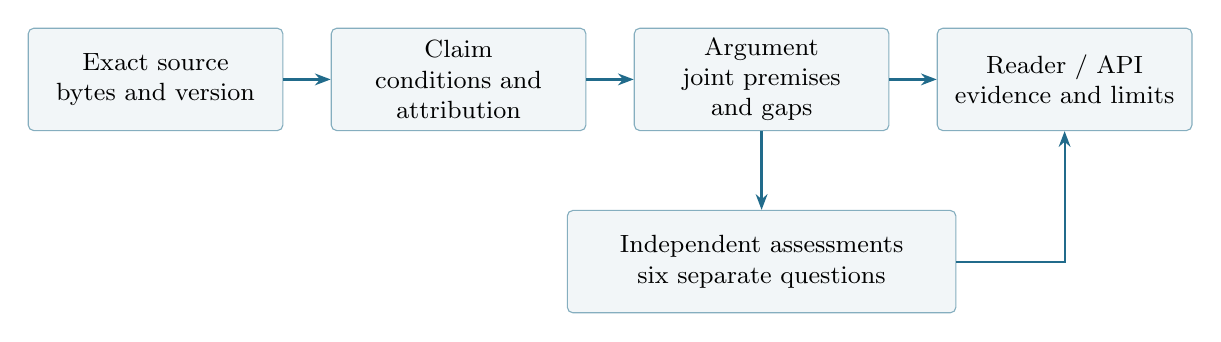
\begin{tikzpicture}[node distance=6mm,box/.style={draw=accent!55,rounded corners=2pt,fill=wash,align=center,text width=30mm,minimum height=13mm,font=\small},link/.style={-{Stealth[length=2mm]},thick,draw=accent}]
\node[box] (source) {Exact source\\bytes and version};
\node[box,right=of source] (claim) {Claim\\conditions and attribution};
\node[box,right=of claim] (arg) {Argument\\joint premises and gaps};
\node[box,right=of arg] (view) {Reader / API\\evidence and limits};
\node[box,below=10mm of arg,text width=47mm] (review) {Independent assessments\\six separate questions};
\draw[link] (source)--(claim);
\draw[link] (claim)--(arg);
\draw[link] (arg)--(view);
\draw[link] (arg)--(review);
\draw[link] (review.east)-|(view.south);
\end{tikzpicture}
\caption{The reading path and evidence path meet at the interface. Arrows in this overview show information flow. They are not themselves mathematical implications. Assessment and publication decisions require their own records.}
\label{fig:overview}
\end{figure}

\subsection{Three related products}

The project produces a protocol, a working implementation and a scientific reading interface. The protocol describes records and constraints; code enforces the implemented subset; the interface helps humans and other programs inspect actual records. A publishable version requires these three products to agree. A field described in a schema does not establish that its producer exists, and an attractive interface cannot supply missing evidence.

The new-paper product path adds an operational requirement: a user submits a new arXiv identifier, the service acquires an exact source version, performs bounded analysis, reports actual task progress and exposes the resulting evidence. This path is more than a replay of a precomputed example. Its first output is a source-grounded candidate view, whose open questions remain visible. Section~\ref{sec:web} separates this operational path from the richer V3 scientific contract.

\subsection{Stable terminology}

\begin{tabularx}{\linewidth}{@{}P{31mm}X@{}}
\toprule
Term & Meaning in this report \\
\midrule
Paper Agent & A versioned, source-bounded collection of records about a paper; not automatically an independently qualified reviewer. \\
Scientific claim & A proposition attributed to a source, preserving scientific conditions and modality. \\
Candidate & A proposed extraction, relation or interpretation whose scientific status has not been admitted by the required process. \\
Assessment & A method-specific conclusion about an exact target, with conditions and evidence. \\
Snapshot & An explicit version boundary defining which records are visible. Its existence does not imply approval. \\
Frontier item & A retained unresolved question, with the affected target and the next evidence needed. \\
API & Application programming interface: the contract by which a program submits work or reads records. \\
\bottomrule
\end{tabularx}

V3 is the architecture version, whereas \ContractVersion{} is the experimental contract version. Software version, API version, paper version, record revision and knowledge snapshot are independent identifiers. The proposed Charter is not currently effective; this report does not ratify it.

\section{Exact identity, sources and claim reconstruction}\label{sec:source}

\subsection{Two hashes answer different questions}

An artifact hash identifies original bytes. A record hash identifies a canonical serialized record. These questions differ: a reformatted JSON file can encode the same canonical record while having different original bytes. Conversely, unchanged paper bytes can support several different candidate interpretations. AgtXIv keeps these identities separate.

\ruleid{I1: exact reference.} A reference to a record binds the tuple
\begin{equation}
  r=(\text{record type},\text{lineage identifier},\text{revision},\text{content hash}).
\end{equation}
The revision is a positive integer. A floating request for the latest version is a convenience query and cannot stand in for this tuple in reproducible evidence. The same lineage and revision cannot be silently reused for changed content.

\ruleid{I2: record envelope.} Each V3 record includes its exact discriminator, identifier, revision, creation time, material class, schema-bundle hash, attributed producer, policy reference, input references, content hash and payload. The canonical record hash excludes only the root \code{content_hash} field. Nested hashes and references remain covered. The implementation uses the existing V2 normalization and integer-safe JSON parser while hashing the V3 flat envelope with its own procedure.

\ruleid{I3: original bytes.} Byte-bearing references bind an artifact identifier, media type, byte size and SHA-256. A filename is a locator, not proof of identity. The local validators reject unresolved references, stale hashes and duplicate identities inside the supplied set. Their scope does not establish that the caller supplied every relevant record in the world.

The bundle manifest binds schema bytes and the offline resolver uses local identifiers. Schema URIs are not instructions to download arbitrary network resources during validation. The generated appendix binds the source manifest used in this report and records the individual input digests in \code{generated/schema-inputs.json}.

\subsection{Acquisition precedes interpretation}

The request identifies the intended paper; acquisition records what was actually obtained. An omitted arXiv version must be resolved and then stored as an exact version for that run. A request, a successful response, a downloaded archive and a published rendering are different observations. Missing source packages, absent supplementary data and unsupported formats require explicit outcomes.

\ruleid{S1: source boundary.} Preserve the selected source bytes and an inventory of the files actually captured. Record their origin and their relationship to the work and version. In the existing robustness example, six original/archive files and eight locally generated build files were all captured. The additional build files were observed artifacts, not evidence that this task executed a paper build.

\ruleid{S2: span boundary.} For text artifacts, byte spans use zero-based, half-open intervals $[a,b)$ over the original bytes. A span binds the parent artifact and selected byte hash. Human-facing line numbers aid navigation but do not replace byte identity. If normalization changes text, retain a transformation record linking its input and output; do not attach normalized offsets to the original artifact.

\ruleid{S3: activity boundary.} TeX is a programmable document format. Static inspection can identify some includes, environments and local references, but does not establish complete macro expansion or published rendering activity. Commented, inactive and unknown material must remain distinguishable. The source pipeline processes data without executing untrusted TeX or scripts.

\subsection{A source claim is not a normalized theorem}

A source-faithful claim retains its statement, source spans, components, conditions, modality, attribution, scientific system and comparison baseline. Mathematical normalization records typed objects, quantifiers, assumptions and conclusions in a separate representation. A component map states which parts were represented mathematically and which scientific meaning remains outside that representation.

\ruleid{S4: preserve meaning.} Dropping a quantifier, changing a physical system, replacing an approximation with an equality or adding a new premise requires an explicit account. A harmless representation correction may remain within a lineage after suitable review; a changed proposition needs a distinct claim identity or explicitly derived claim. Neither a text similarity score nor a matching hash is an oracle for semantic identity.

\ruleid{S5: freeze the denominator.} An inventory records discovered claims, non-claim material and unknown content. A frozen scope binds a reviewed inventory and the required work. A later failure cannot be hidden by deleting an obligation. Corrections to omissions, additions of work and new scientific hypotheses follow different revision paths, with old records retained.

\boundary{A lexical candidate inventory is a reproducible reading aid. Its number of lines, spans or cues is not a count of scientifically distinct propositions, and complete byte coverage does not establish complete semantic discovery.}

\section{Arguments and six separate assessment questions}\label{sec:assessment}

\subsection{Joint premises and local assumptions}

An argument is represented through nodes, inference steps, assumption contexts, proof routes and explicit dependency bindings. A joint inference has the form
\begin{equation}
  (P_1,\ldots,P_k;\Gamma,\mathcal{R})\Longrightarrow Q,
\end{equation}
where $\Gamma$ names the local assumptions and $\mathcal{R}$ the stated rule. This representation preserves the fact that the premises are used together. Drawing independent arrows $P_i\to Q$ without recording their joint use can incorrectly suggest that each premise alone proves the conclusion.

\ruleid{A1: distinguish graph meanings.} Document containment, provenance, mathematical dependence and scientific comparison are different relations. A heading containing a theorem is not a proof dependency. A paper citing another paper does not by itself identify a load-bearing theorem. The interface must expose relation type and candidate status before relying on graph reachability.

\ruleid{A2: preserve context.} A statement proved under a local assumption cannot escape that context merely because a producer labels the assumption discharged. The implemented record checks constrain supported discharge forms and evidence references, but do not themselves prove every inference rule. Alternative proof routes remain separate, so a gap in one route does not automatically negate another.

The pinned vibefeld adapter illustrates another boundary: replaying supplied ledger bytes and comparing them with an export can establish internal consistency of that capture. It does not authenticate declared identities or establish that an independent upstream process actually ran. Upstream labels such as \code{validated}, \code{clean}, \code{closed} and \code{admitted} remain attributed reports. They are not V3 scientific approval or knowledge admission.

\subsection{What the six axes ask}

\begin{longtable}{@{}P{37mm}P{58mm}P{24mm}@{}}
\toprule
Axis & Scientific question & Example evidence \\
\midrule\endfirsthead
\toprule Axis & Scientific question & Example evidence \\
\midrule\endhead
Source fidelity & Does the recorded proposition preserve what the source says, including attribution and conditions? & Exact spans and source review \\
Mathematical correctness & Does the stated mathematical conclusion follow under the recorded assumptions? & Argument review or suitable formal evidence \\
Formal alignment & Does the formal statement express the intended mathematical target? & Exact endpoint comparison and backtranslation \\
Semantic applicability & Do mathematical objects, assumptions and approximations apply to the scientific use under discussion? & Model and domain review \\
Empirical support & Do observations support the scientific claim under the stated methodology and uncertainty? & Data and empirical review \\
Computational reproducibility & Can the specified computation be reproduced under its input, environment and comparison protocol? & Execution records and reproduction review \\
\bottomrule
\end{longtable}

\ruleid{A3: no automatic transfer.} Lean kernel success concerns a formal declaration in an environment. It does not, alone, establish source fidelity, correct translation, physical applicability or empirical support. Similarly, reproducing a plotted numerical value does not establish that the experiment supports the physical interpretation assigned to it.

\subsection{Applicability, conclusion and execution}

Each axis assessment separates three state dimensions. Applicability asks whether the question applies: \code{UNDETERMINED}, \code{APPLICABLE} or \code{NOT_APPLICABLE}. Result records the evidence conclusion: \code{NOT_ASSESSED}, \code{INCONCLUSIVE}, \code{PARTIALLY_SUPPORTED}, \code{SUPPORTED} or \code{COUNTEREVIDENCE}. Execution records what work occurred: \code{DEFERRED}, \code{BLOCKED}, \code{FAILED} or \code{COMPLETED}. A method, exact targets, review context, supporting and opposing evidence, conditions and unresolved frontiers accompany these labels.

\ruleid{A4: retain disagreement.} A status view is a read-only projection over a supplied record set. It must preserve differing assessments of the same exact target, including their conditions and methods. Selecting the newest positive assessment while hiding an earlier relevant objection is not an acceptable reduction. Missing evidence is not zero evidence, and an unmeasured quantity is not a measured zero.

The local \code{project_axes} function retains the assessments of the exact target in the supplied collection. A serialized \code{StatusView} is a separate record whose validation checks implemented bindings; it is not a mechanical proof that its author supplied every assessment. Neither mechanism establishes completeness outside the submitted record universe.

\ruleid{A5: distinguish success from accounting.} A work obligation can be accounted for by a documented failure or deferral where its processing profile permits this. An obligation marked \code{SUCCESS_REQUIRED} additionally needs suitable success evidence for the exact target. Filling a result-reference field with an arbitrary existing record cannot discharge that requirement. Unsupported completion stages remain fail-closed in the local implementation.

\subsection{Independence is more than a different name}

Review records bind who reviewed what, which inputs were visible and the applicable policy. The local \code{AuthorityContext} is an explicit capability supplied by a trusted integrating caller. It can check aliases, visible inputs, named roles and allowed policies within that boundary. A self-authored identity file is not independent authentication, and different agent names do not establish independent institutions or uncorrelated reasoning.

\ruleid{A6: do not promote validation output.} A consistent candidate graph may legitimately report that authority was not checked. Such output is not a release token. Formal scientific decisions require the adopted qualification and separation policies, actual execution evidence where applicable, and appropriate domain review. These institutional and scientific requirements are not supplied by the schema package.

A precise formal expression can align with an intended mathematical target before its proof is complete. Conversely, kernel acceptance cannot rescue a formal statement that expresses a different target. Formal-alignment evidence must therefore name the actual comparison endpoints, rather than borrowing a source-to-argument review that never compared the formal representation.

\section{Record families across the lifecycle}\label{sec:lifecycle}

The \RecordFamilyCount{} V3 record families cover a planned lifecycle rather than \RecordFamilyCount{} running services. The groups below explain why each family exists and where it hands information to another stage. Appendix~\ref{app:fields} supplies the generated payload and shared-field reference. The groups are an explanatory organization; exact discriminators and references remain those of the schemas.

\subsection{Policy and evidence planning: three families}

\textbf{ProcessingProfile, AuthorityPolicy, EvidenceProtocol.} A processing profile specifies required stages, axes, success obligations and permitted unresolved outcomes. Authority policy records governance state, role separation, identity requirements and human-review triggers. Evidence protocols state a comparison plan before the result being assessed is selected. Their shared purpose is to make the acceptance question explicit in advance; an authored policy record does not adopt itself.

\subsection{Acquisition and source representation: six families}

\textbf{SourceRequest, SourceAcquisition, SourceSnapshot, SourceSpan, SourceTransformation, PaperStructure.} The request expresses intent, acquisition records its actual outcome, and the snapshot binds acquired material. Spans locate specific bytes, transformations describe changed representations, and paper structure records document relationships. This separation allows an acquisition failure or uncertain rendering status to remain visible without destroying the request or inventing source content.

\subsection{Inventory, scope and obligations: five families}

\textbf{AgentizationPlan, InventoryDiscovery, ScopeFreezeDecision, FrozenInventoryScope, ObligationDisposition.} The plan proposes work; discovery records what the source inventory actually contains; an independent scope decision may freeze that work under a profile. Each frozen obligation has a current disposition while historical attempts remain available. Scope is a versioned scientific boundary, not an adjustable progress-bar denominator.

\subsection{Scientific and mathematical meaning: seven families}

\textbf{ScientificClaim, DerivedClaim, ClaimComponentMap, SemanticContext, MathematicalDefinition, MathClaimIR, AssumptionContext.} These records separate attributed source propositions from system-derived propositions, retain the component correspondence, and describe mathematical and scientific context. MathClaimIR means mathematical claim intermediate representation. A definition can be reused only under a compatible meaning and version. Assumption contexts are explicit so that a conditional derivation can be displayed without silently turning into an unconditional claim.

\subsection{Arguments and work history: eleven families}

\textbf{ArgumentNode, InferenceStep, ProofPlan, DependencyBinding, Challenge, ChallengeDisposition, ArgumentSnapshot, ArgumentReview, UpstreamImport, WorkAttempt, WorkCompletion.} Nodes and joint inference steps represent an argument; proof plans distinguish routes; bindings identify exact dependencies. Challenges and their dispositions preserve objections and responses. A snapshot supplies a recoverable argument boundary. Imports retain upstream attribution, while attempts and completions retain reported or observed work evidence. Establishing actual execution requires suitable independently supplied receipts. A reply does not automatically resolve a challenge, and a worker completion does not itself establish a theorem.

\subsection{Formalization and assessment: twelve families}

\textbf{FormalEnvironment, FormalizationPacket, FormalizationAttempt, FormalCheckRecord, BacktranslationRecord, AlignmentAssessment, EmpiricalEvidence, ReproductionRecord, AxisAssessment, StatusView, CounterexampleRecord, EnvironmentCompatibility.} A formalization packet binds a target and context. An attempt records attributed production; a check binds reported or observed evidence to declared targets and an environment. Independent execution receipts are needed to establish which checks actually ran. Backtranslation and alignment inspect meaning at exact endpoints. Empirical and computational evidence remain separate. Counterexamples specify what they contradict; environment checks support a proposed use. A status view aggregates these records without changing their targets or authority.

\subsection{Knowledge comparison and reuse: five families}

\textbf{BaselineSnapshot, RelationAssessment, ContributionDelta, ReuseDecision, FrontierItem.} A contribution is relative to an explicit baseline. Relations such as equivalence, restriction, extension or refutation require the appropriate endpoint comparisons and evidence. A new proof of a known theorem can be a method contribution without becoming a new theorem; a textually different formulation may add no supported result. Reuse decisions are use-specific and preserve assumptions, environment and conflicts. Frontier items retain the work required before a future decision becomes possible.

\subsection{Package, archive and admission: eight families}

\textbf{PaperAgentManifest, ReleaseAudit, ReleaseCertificate, PaperAgentRelease, ArchiveReceipt, AdmissionDecision, KnowledgeSnapshot, KnowledgeIngestionReceipt.} The manifest fixes candidate contents; audit and mechanical certification bind that exact manifest; a paper release fixes the resulting package. Archiving preserves the release. A later admission decision selects eligible records for a knowledge snapshot, and an ingestion receipt records the actual transaction. Software merge, package release, archive and knowledge admission are separate events. A successful database write is not an independent scientific review.

\subsection{History, migration and observation: seven families}

\textbf{EventRecord, EventCheckpoint, ImpactAnalysis, RevisionRecord, LegacyBinding, QueryReceipt, EvaluationReport.} Events and checkpoints retain operational history. Impact analysis identifies potentially affected records along declared dependencies without rewriting old assessments. Revision records preserve changes; legacy bindings retain the source contract of older material. Query receipts bind what was returned under a snapshot. Evaluation reports record measured scope, baselines and limitations rather than converting absent measurements into favourable results.

\subsection{Local implementation boundary}

The current Python modules implement offline schema and supplied-record validation, local source inspection, frozen-obligation checks, a pinned upstream capture parser, potential dependency analysis and bounded SQLite candidate storage. The local store validates an input set before committing, preserves immutable object identities and can update a provisional head with compare-and-swap. That operation changes the head only if it still equals the expected previous value, preventing a stale writer from silently replacing a concurrent update.

Historical queries resolve exact records and retain known relevant conflict endpoints. Their responses remain provisional. The implementation trusts its local filesystem and integrating process; it is not a production identity provider, externally witnessed archive or formal admission service. The richer release and scientific lifecycle families remain necessary interfaces even where only their shape and some cross-record rules are currently implemented.

\section{Worked example: robustness of magic}\label{sec:robustness}

\subsection{What is being reconstructed}

Howard and Campbell define robustness of magic through signed decompositions into pure stabilizer states and state its monotonicity under trace-preserving stabilizer channels~\cite{howard2016magic}. The local source-grounding note identifies the definition, the R3 statement, its proof steps and a separate postselection extension. This section explains the recorded argument and its assumptions; it is not a new independent scientific certification.

For a finite multiqubit system, let $\Stab_n=\{\sigma_i\}$ denote the pure stabilizer projectors used as decomposition atoms. A density operator $\rho$ has a real signed decomposition
\begin{equation}
  \rho=\sum_i x_i\sigma_i,
  \qquad \sum_i x_i=1,
  \qquad x_i\in\mathbb{R}.
\end{equation}
The coefficients need not be probabilities: some can be negative. The source defines
\begin{equation}
  \RoM(\rho)=\min_{\{x_i:\rho=\sum_i x_i\sigma_i\}}\sum_i|x_i|.
  \label{eq:robustness}
\end{equation}
The total absolute coefficient weight measures how much signed weight is needed to represent the state in these free atoms. An ordinary convex mixture has total weight one. The technical obligation to establish feasible decompositions and attainment of the minimum is separate from writing down this definition.

\subsection{Why trace preservation gives the contraction}

For the selected R3 argument, assume linearity and that the channel maps every input stabilizer atom to a nonnegative, normalized mixture of output stabilizer atoms:
\begin{equation}
  \mathcal{E}(\sigma_i)=\sum_j p_{ij}\sigma_j,
  \qquad p_{ij}\geq0,
  \qquad\sum_jp_{ij}=1.
  \label{eq:channel}
\end{equation}
This is mixture preservation, not the stronger claim that every input atom maps to a single atom. It is therefore important to keep the two indices and normalization condition in the recorded mathematical target.

Take an optimal input decomposition $x$. Linearity and regrouping give the feasible output decomposition
\begin{equation}
  \mathcal{E}(\rho)=\sum_jx'_j\sigma_j,
  \qquad x'_j=\sum_ix_ip_{ij}.
\end{equation}
The definition, triangle inequality, nonnegativity and row normalization yield
\begin{align}
  \RoM(\mathcal{E}(\rho))
  &\leq\sum_j\left|\sum_ix_ip_{ij}\right|\nonumber\\
  &\leq\sum_{i,j}|x_i|p_{ij}\nonumber\\
  &=\sum_i|x_i|\underbrace{\sum_jp_{ij}}_{1}\nonumber\\
  &=\RoM(\rho).
  \label{eq:contraction}
\end{align}
The final equality uses optimality of the input decomposition. For an arbitrary feasible $x$, the preceding argument gives only the upper bound $\sum_i|x_i|$, which may exceed $\RoM(\rho)$. An alternative proof could use an infimum and a limiting argument, but that is a distinct reconstruction with its own obligations.

The physical picture is simple: a free operation redistributes each signed input weight among free output atoms using nonnegative proportions that sum to one. Redistribution cannot increase the total absolute weight, and cancellations can reduce it. The assumptions in Eq.~\eqref{eq:channel} are precisely what makes this picture match the algebra.

\subsection{Why postselection is a separate claim}

A selected measurement branch is represented before normalization by a trace-nonincreasing map $\mathcal{E}_b$. Its success probability is
\begin{equation}
  q_b=\Tr\mathcal{E}_b(\rho),\qquad
  \rho_b=\mathcal{E}_b(\rho)/q_b\quad(q_b>0).
\end{equation}
Normalization divides by a state-dependent probability. The row sums used in Eq.~\eqref{eq:contraction} are no longer all one for an individual branch. The trace-preserving proof therefore does not directly show $\RoM(\rho_b)\leq\RoM(\rho)$ for each normalized selected outcome.

The source separately discusses an average/postselection extension and points to another argument. A probability-weighted quantity, such as an average over outcomes, asks a different question from the robustness of a single conditional branch. AgtXIv keeps this assertion on a separate route with its own source span and open obligations; it does not count it as discharged by R3.

\subsection{Exact anchors and observed evidence}

\begin{tabularx}{\linewidth}{@{}P{33mm}P{25mm}X@{}}
\toprule
Source segment & TeX lines & Original byte interval \\
\midrule
Definition & 75--79 & \code{[9218,10126)} \\
R3 statement & 225 & \code{[33249,33406)} \\
Channel action & 251--255 & \code{[35064,35619)} \\
Output mixture & 256--259 & \code{[35619,35847)} \\
Norm contraction & 260--265 & \code{[35847,36153)} \\
Separate extension & 266 & \code{[36153,36418)} \\
\bottomrule
\end{tabularx}

The original TeX is \code{Robustness_main_appendix.tex}, SHA-256 \code{48adf581a5f8353bb1125c75b8e0a075ff7ba79917f2a12d9f7e0f4ad1a8312d}. These anchors were read from the retained source and source-review note. The historical candidate capture contains 14 files totalling 1,542,636 bytes. Its 548 main-text lines were assigned 240 tentative claim cues, 204 non-claim cues and 104 unknown-text items. These numbers describe lexical coverage, not scientific claim counts.

The recorded output contains 35 candidate records, one unadopted context policy, six proposed interpretations, five dependency bindings, twelve frontier items and nine open/deferred candidate obligations. A fresh database import, a separate-process read-only reopen and byte-identical replay under the same known observation were recorded. No formal frozen scope, scientific assessment or knowledge admission was produced. Supplementary numerical matrices and solver evidence referenced by the paper were not found in the inspected source package; this observation does not establish their absence from every remote location.

\boundary{The candidate chain can expose the optimal-decomposition assumption and keep postselection separate. This is evidence of useful representation and traceability. The mathematical obligations, source-to-formal alignment, full-paper semantic coverage and formal scientific admission remain open in this V3 candidate record.}

\section{New-paper web and API architecture}\label{sec:web}

\subsection{Purpose and implementation status}

The release interface must accept a new arXiv paper and perform a real bounded analysis. This operational requirement is distinct from the precomputed V1 demonstration and from independent scientific assessment. The primary user path is submission, acquisition, processing, visible progress or failure, and a result linked to source evidence. A successful run may still report incomplete extraction or no supported scientific conclusions.

\boundary{The routes and state behaviour below are bound to the local implementation and an actual HTTP submission of HepLean, arXiv:2405.08863v1. The retained verification covers task/result schemas, exact-version acquisition, repeated result reads and six unassessed axes. Local browser checks additionally cover real submissions, refresh recovery, narrow-screen layout and keyboard interaction. Public deployment remains a separate release check.}

The selected implementation uses a plain HTML, CSS and JavaScript front end under \code{web/}, with an ECMAScript-module Cloudflare Worker as the server. D1 stores task metadata and stage transitions; R2 retains acquired source bytes and generated results. An independent intake module performs arXiv input handling, real acquisition, bounded archive and TeX parsing, candidate source-span extraction and local-reference dependency extraction. These are source-processing operations; no language-model scientific approval is supplied by this path.

\begin{figure}[htbp]
\centering
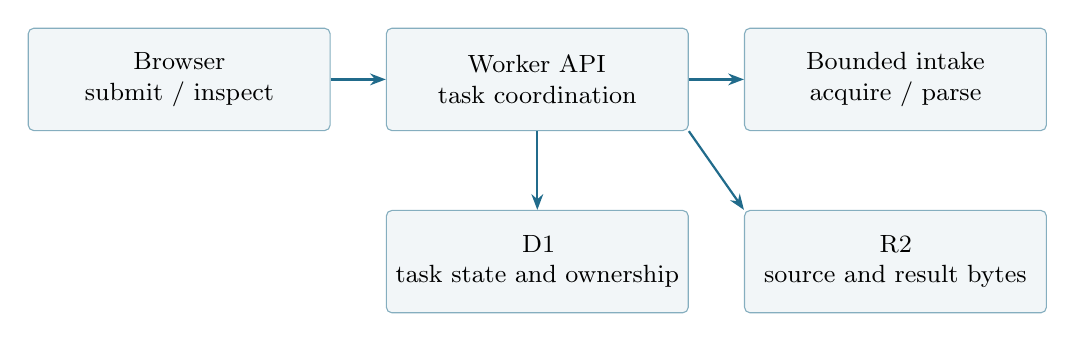
\begin{tikzpicture}[node distance=7mm,box/.style={draw=accent!55,rounded corners=2pt,fill=wash,align=center,text width=36mm,minimum height=13mm,font=\small},link/.style={-{Stealth[length=2mm]},thick,draw=accent}]
\node[box] (browser) {Browser\\submit / inspect};
\node[box,right=of browser] (worker) {Worker API\\task coordination};
\node[box,right=of worker] (intake) {Bounded intake\\acquire / parse};
\node[box,below=10mm of worker] (d1) {D1\\task state and ownership};
\node[box,below=10mm of intake] (r2) {R2\\source and result bytes};
\draw[link] (browser)--(worker);
\draw[link] (worker)--(intake);
\draw[link] (worker)--(d1);
\draw[link] (worker.south east)--(r2.north west);
\end{tikzpicture}
\caption{Operational architecture for new-paper processing. Task metadata and byte objects serve different roles. Cross-service failures require explicit recovery; this diagram does not imply a single atomic transaction across D1 and R2.}
\label{fig:web}
\end{figure}

\subsection{Required transport contract}

The API has a major-version path prefix \code{/api/v1} and currently returns \code{api_version: "1.0"}. The inspected routes are:

\begin{longtable}{@{}P{62mm}P{76mm}@{}}
\toprule
Operation & Request and response meaning \\
\midrule\endfirsthead
\toprule Operation & Request and response meaning \\
\midrule\endhead
GET \code{/api/v1/health} & Service configuration state: \code{READY} if both stores are bound, otherwise \code{READ_ONLY}; no scientific assessment. \\
GET \code{/api/v1/library?q=...} & Curated paper records, optionally filtered by a case-insensitive query of at most 200 characters. This endpoint returns the selected finite library, not a paginated global arXiv index. \\
GET \code{/api/v1/papers/SLUG} & One curated paper, or 404. A missing curated paper can be submitted through the jobs endpoint. \\
GET \code{/api/v1/schemas} & The exposed schema catalog and its bundle identity. \\
POST \code{/api/v1/jobs} & JSON object with exactly one string field, \code{arxiv}. Returns 202 with a task view and \code{Location} pointing to the task. \\
GET \code{/api/v1/jobs/JOB_ID} & Persisted task view: state, timestamps, revision, parent, result location and structured error where applicable. \\
GET \code{/api/v1/jobs/JOB_ID/result} & Completed result bytes; 409 before completion; 503 for a missing or hash-mismatched retained result. \\
POST \code{/api/v1/jobs/JOB_ID/retry} & Empty JSON object. Only failed or interrupted tasks are retryable. Creates a new task with \code{parent_id}; it does not overwrite the previous attempt. \\
\bottomrule
\end{longtable}

The capitalized segments \code{SLUG} and \code{JOB_ID} are route variables, not literal path components. JSON requests are limited to 2 KiB and require \code{application/json}. Cross-origin browser POST requests are rejected. Error responses contain a code, message and request identifier; a successful transport status does not imply a supported scientific claim.

\ruleid{W1: submit intent.} The submission request contains exactly the \code{arxiv} field, accepting an arXiv identifier or recognized arXiv URL; no processing-options field is currently supported. The server validates and normalizes the identifier before acquisition. An arbitrary user-supplied URL is not an authorized fetch destination. The response supplies a stable task identifier and the means to inspect its state. The acquired version and source identity are recorded separately from the requested identifier.

\ruleid{W2: report actual state.} A task exposes its current stage, update or revision identity, and structured errors. Progress reflects persisted work transitions rather than a client-side timer. Concurrent attempts must not both take ownership of the same stage; a compare-and-swap transition checks the expected state before changing it. Interrupted or expired attempts require an explicit retry/recovery policy rather than indefinite apparent progress.

The persisted success sequence is \code{QUEUED} $\to$ \code{FETCHING} $\to$ \code{ANALYZING} $\to$ \code{COMPLETED}, with \code{FAILED} for a recorded processing failure. A non-terminal task with no update for more than 120 seconds is projected as \code{INTERRUPTED} when read. This derived view does not rewrite its stored state or confirm that the worker has stopped. The earlier attempt may still complete. A retry records a separate task and parent link, preserving both attempts and their possible results. All task views explicitly report \code{scientific_assessment: "NOT_PERFORMED"}.

\ruleid{W3: retain evidence.} Results bind the resolved source identity, original byte digest, processing version, extraction limits, candidate records and warnings. Candidate relations preserve their extraction basis. A local TeX reference is evidence of an explicit textual reference; it is not automatically a validated mathematical implication. Reading a job result must not mutate its source record or scientific status.

Source archives are retained privately under keys derived from their SHA-256. Result JSON is likewise stored under its own byte digest, which is checked on result retrieval. A source digest and a result digest identify different byte objects. The result includes requested and resolved source information, retrieval time, archive digest, engine version, candidate spans and explicit remaining limitations. In the HTTP result, \code{transport.archive_sha256} uses the \code{sha256:} prefix required by the response schema. Candidate assessment entries remain \code{NO_ASSESSMENT}; they are not V3 \code{AxisAssessment} records.

\ruleid{W4: expose failure.} Invalid input, unknown work, source unavailability, unsupported source format, archive rejection, resource limits and processing failure need separate error codes or documented details. An error response must not expose internal credentials or arbitrary filesystem paths. The client displays which stage failed and whether retry is meaningful. A failed parse must not leave a successful-result label.

\ruleid{W5: document the actual interface.} The OpenAPI 3.1 description is published as a build artifact at \code{web/public/api/v1/openapi.json}, exposed at \code{/api/v1/openapi.json}. It defines routes, methods, request/response schemas, status codes and polling/retry semantics. The strict intake result schema is maintained at \code{src/agtxiv_web/analysis.schema.json}. Task retention and production access policy still require operational decisions. The task-result contract remains distinct from V3 scientific records; similar field names do not make an operational JSON object a sealed V3 record.

\subsection{Bounded processing and separation from scientific work}

Input acquisition must constrain network destinations, redirects, response size and time. Archive processing must constrain expanded bytes, entry count, path traversal, links and malformed members. TeX inspection is static and must not execute source-controlled commands. The configured limits belong in API documentation and actual server-side checks, not only in front-end validation.

The server uses a 20-second configured timeout for both acquisition and analysis, and a conditional update to a shared submission clock permitting a new task no more often than every 3.5 seconds. A conditional SQL insertion admits a task only while fewer than three non-terminal tasks have recent updates. The 120-second cutoff bounds recently active records, not every worker that may still run after a stale projection. Intake bounds downloads to 8 MiB, expansion to 16 MiB, one file to 2 MiB, total TeX text to 4 MiB, tar entries to 1,024, files to 512 and candidates to 240. Other limits bound labels, references, includes, structural spans and hashing work. Each result records the configured limits under its defined response schema. Earlier browser receipts retain their original 30-second engine field; the final HTTP receipt records the current 20-second configuration.

Source-span candidates provide a route from a displayed item to the bytes examined. They do not establish complete semantic claim discovery, source-faithful paraphrase or theorem validity. If a run cannot resolve macros, parse a document class or interpret a figure, that uncertainty belongs in the result. Restricting work is acceptable when the limit is explicit; reporting that limited work as complete scientific analysis is not.

The web service therefore has its own operational lifecycle, while V3 describes a richer scientific lifecycle. D1 and R2 here serve the bounded web task implementation. Their use does not silently adopt or replace the V2 production authority proposal, which distinguishes reviewed Git material, canonical replay bundles, operational transactions and disposable projections. A future adapter must bind a task's actual artifacts, producer and evidence to the relevant V3 records before any stronger scientific interpretation is made.

\subsection{Reader and interface acceptance}

A reader should be able to submit a new paper, inspect a persisted task after refreshing the page, open the result, locate a source passage and identify missing evidence. The graph must distinguish workflow steps from paper-specific dependencies. Keyboard navigation, visible focus, narrow-screen layout, readable formulas and text labels for status colours are part of the acceptance path.

The signed-weight interaction accompanying R3 is an algebraic illustration of nonnegative redistribution and cancellation. Its displayed coefficients and transition matrix are not a specified quantum state and channel, and its total absolute weight is not a computed state robustness. The interface must keep this distinction visible alongside the optimal-decomposition and trace-preserving assumptions.

Final integration checks must include a new paper outside the precomputed example list, actual source acquisition, result evidence, a meaningful failure case, persisted task lookup and an independent comparison of API and displayed states. Successful local checks are not evidence of public deployment; the release record must name the actual running location or provide an explicitly local run procedure.

The local adapter in \code{web/dev.mjs} uses Node's SQLite support and a private local object directory to exercise the same handler. Its default address is \code{http://127.0.0.1:8787}. It is a development environment, not a measurement of the production Cloudflare deployment. The server entry point can be started from the repository root with \code{node web/dev.mjs} after the required runtime and web assets are available.

\subsection{Retained live HTTP evidence}

The local run recorded in \code{docs/evidence/publishable-release/heplean-http-final/verification.json} submitted \code{2405.08863v1} to the running HTTP service on 7 September 2026 at 23:03 UTC. It observed \code{QUEUED}, then \code{COMPLETED} with revision 3, and retrieved identical result bytes twice. Polling did not capture each intermediate stage separately. The exact version 1 archive contains three source files, including two TeX files; the extractor returned 15 candidates. All six axes remained \code{NO_ASSESSMENT}, and \code{scientific_acceptance} remained false.

The receipt reports successful job-schema, full result-schema, exact-version, retained-source, repeated-read and six-axis checks. The result in \code{heplean-http-final/result.json} has a nonempty entity tag matching its byte digest and reports \code{limits.timeoutMs=20000}. Earlier receipts remain historical evidence. These checks establish a real processing path, not extraction accuracy or scientific endorsement of HepLean.

Browser checks initially exposed an incorrect MIME type for the root HTML page, observed as \code{ERR_BLOCKED_BY_CLIENT}. The root response was corrected to \code{text/html} and a regression test added. The local browser then rendered the white interface and completed a form submission of HepLean with 15 candidates and three source files. The browser's two exposed WebMCP tools were discovered; reading the submitted task agreed with the API, a new tool submission of \code{1706.03762} resolved to version 7 and completed with 11 candidates and 23 inventoried source files, and an invalid external URL was rejected by both tool and form paths.

The receipt \code{docs/evidence/publishable-release/browser-verification.json} records these checks and additional refresh recovery, keyboard interaction with the signed-weight slider, real schema-field expansion and absence of captured browser errors. A 390-by-844 viewport override produced equal measured client and document-scroll widths of 375 pixels, with no page-wide horizontal overflow in the inspected flow. This is scoped local interface evidence, not a complete accessibility audit. The retained task/result JSON files accompany the receipt under \code{browser/}. Report-download verification and an actual public deployment URL remain separate next steps.

A separate local handler check submitted 20 concurrent same-origin requests: one received 202, nineteen received 429, and one processing task was scheduled. Its receipt is \code{docs/evidence/publishable-release/intake-checks/concurrency-local.json}. This check injected a synthetic TeX upstream and used the local SQLite adapter; it tests the observed admission behaviour, not Cloudflare production concurrency or real upstream throughput. The accompanying retained logs report 14 engine tests, 23 response-schema tests and six handler tests passing. These scoped results do not replace a full repository or production release check.

\section{Implementation evidence, maintenance and release}\label{sec:release}

\subsection{What has been checked}

The historical \code{docs/evidence/v3-real-candidate/verification.json} records 710 V3 tests with no failures, errors or skips on 7 September 2026. Its scope also includes 70 generated package files, the pinned upstream protocol, bundle validation, compilation and 106 unchanged historical inputs. These figures do not certify the current release.

Rejection tests cover malformed or stale identities, escaped assumptions, conditional promotion, unsupported reuse, misleading evidence wrappers, historical forks and transaction recovery. They constrain incorrect bindings in supplied records; they do not measure semantic extraction accuracy or establish independent scientific review.

Current HTTP evidence is scoped in Section~\ref{sec:web}. The aggregate gate encountered a pre-existing dirty frozen-baseline mismatch against \code{HEAD}, rather than a newly failing test. The independent full test run was outstanding at this checkpoint. Historical tests and local HTTP success do not complete that gate. Report compilation and packaging have a separate receipt at \code{docs/evidence/publishable-release/report-validation.json}.

\begin{tabularx}{\linewidth}{@{}P{35mm}X@{}}
\toprule
Evidence & Appropriate interpretation \\
\midrule
Schema/record validation & The implemented constraints hold for the supplied objects and exact bundle. \\
Parser/source tests & Bounded input handling and selected source-location behaviours match the tested cases. \\
Candidate replay & The recorded local observation can be re-read or replayed with the stated byte identity. \\
Historical Lean evidence & Only its named declaration, environment, premise and alignment scope; not all V3 scientific obligations. \\
Browser/API test & The tested user operation reaches the recorded service result; not scientific approval. \\
\bottomrule
\end{tabularx}

\subsection{Compatibility and document authority}

\ruleid{M1: preserve old contracts.} V1 and V2 records retain their original schema and evidence scope. The root pilot release manifest is historically \code{accepted_release=false}; its scientific release gate is blocked. That state is not changed by introducing V3 schemas or a new website. A legacy adapter can expose older records with explicit version labels, but cannot turn three old assessment dimensions into six newly assessed dimensions.

\ruleid{M2: make authority visible.} The V3 proposal, V1/V2 specifications, pending Charter, research studies and implementation receipts serve distinct roles. This report describes implementation and maintenance; it does not ratify the Charter. Its appendix derives fields from the bound schemas rather than redefining them.

The existing static Pages builder previously selected the old mathematics-pipeline demonstration, while newer visual prototypes and V3 candidates were outside that path. Publication must verify the actual assembled entry point, not merely the existence of a new page in the repository. The new service also requires a running processing backend; a static website alone cannot fulfil the new-paper analysis requirement.

\subsection{Recoverable repository organization}

\ruleid{M3: preserve before cleaning.} A cleanup first records original paths, destinations, sizes, hashes and reasons. Unique historical byte stores require preservation before deleting temporary files. Fixed historical evidence is not rewritten to conceal changed paths or inputs. A new relocation record explains where unchanged bytes can be found.

The first organization pass copied five complete candidate-history files from the temporary capture directory to an ignored \code{local-archive/} directory and kept the originals. The destination bytes matched the historical closure receipt; both SQLite copies passed a read-only structural quick check. Four historical presentation exports were moved from the repository root into \code{docs/archive/presentations/2026-08/}. The nine archived files total 16,488,328 bytes. The archive manifest records exact hashes and reversible path mappings.

A second pass moved 17 files from the two superseded interface prototypes into \code{docs/archive/prototypes/}. Three README files gained explicit relocation notes; other file bytes were unchanged, and the original README content remains recoverable as verified prefixes. The combined manifest has 26 entries and 18,943,027 destination bytes. Local prototype resources, anchors and graph-data references were checked after relocation.

The operation left scientific source caches, fixed reference inputs, active slides, schema packages and Lean caches untouched. The local copy reduces the risk of losing historical evidence during temporary-directory cleanup; it is not an off-device backup or independent tamper-proof archive. Archiving material locally does not grant permission to redistribute it in a public website or release.

\subsection{Build and release procedure}

\ruleid{R1: bind the candidate.} Record the exact source revision, dependency locks, generated-input identities, migration notes and output digests. Separate the software version from record contracts, API version and paper releases. A clean reproducible build is a software property, not scientific acceptance.

\ruleid{R2: run appropriate checks.} The release check set should include the repository aggregate validation, schema and upstream-generation drift checks, V3 contract checks, the new intake's resource and failure tests, API/task integration, browser acceptance and report compilation. A known blocker is reported as such, rather than silently skipped or counted as a scientific pass. Expensive formal builds use their defined environment and scope.

\ruleid{R3: publish the intended bytes.} Build the website and service from the reviewed candidate. Verify deep links, downloads, subpath behaviour, error states and the actual deployed endpoint when deployment occurs. Public artifacts must be selected deliberately; local research caches and preserved byte stores are not default release content. Root licence, contributor and production-governance decisions remain governed by the project's actual policies.

\ruleid{R4: preserve operations.} Document service configuration, data retention, access boundaries, failure recovery and backup/restore procedures. Recovery must account for both task metadata and byte objects. A task that points to a missing result needs an explicit repair path, and an unreferenced byte object needs a retention policy. Production durability and throughput require separate measurements.

\ruleid{R5: retain an honest handoff.} The authorized work window ends at 03:00 Europe/Amsterdam on 8 September 2026, equivalent to 01:00 UTC. Work remaining at that deadline is saved with concrete files, evidence, failure reasons and next operations. The deadline does not make an unfinished implementation or scientific task complete.

\subsection{Reproducible report commands}

The report appendix generator reads the source schemas and writes only its own generated files. It exposes a no-write comparison mode. From the repository root:
\begin{lstlisting}
.venv/bin/python docs/technical-report/generate_appendix.py
.venv/bin/python docs/technical-report/generate_appendix.py --check
bash docs/technical-report/build.sh
\end{lstlisting}
The PDF is written to \code{docs/technical-report/build/main.pdf}. Build intermediates are ignored. A portable source archive includes the TeX, BibTeX, generated appendix and build script. Outside the repository, \code{bash build.sh --frozen-appendix} compiles that included snapshot without claiming to check drift against absent schema inputs. The default repository build retains the generation check. The layout is rendered and reviewed separately from compilation, because successful TeX execution does not guarantee readable tables or diagrams.

\section{Boundaries, evaluation and next work}\label{sec:discussion}

The current result makes scientific work traceable while checking selected misbindings. The robustness example explains the need: trace preservation, optimal decomposition and postselection each change the argument and must remain inspectable.

Lexical cues do not establish complete semantic coverage, byte identity does not establish faithful interpretation, review fields do not authenticate independence, and local transactions do not establish production durability. Intake supplies candidates while these scientific and operational questions remain open.

Future evaluations need fixed papers, scope and evidence standards. Useful measurements include omitted conditions, correct source locations, rejected misuse, resolution time and recovery. Efficiency claims require a measured baseline. The original 58-task roadmap remains in force; the seven-workstream release plan does not discharge unperformed scientific work.

\subsection{Claim--evidence map}

{\small
\begin{longtable}{@{}P{43mm}P{69mm}P{34mm}@{}}
\toprule
Claim & Source of evidence & Status in this report \\
\midrule\endfirsthead
\toprule Claim & Source of evidence & Status in this report \\
\midrule\endhead
64 record families and 19 shared structures & Bound catalog, shared schema and generated appendix inventory & Directly enumerated \\
Six questions are represented separately & Axis schema, projection code and invariant ledger & Contract/local mechanism \\
R3 assumptions and norm contraction & Original TeX and exact source-review anchors & Source-grounded reconstruction \\
Historical candidate rereading & Closure receipt and retained database bytes & Historical local check \\
710 V3 tests passed at the stated checkpoint & Stored verification JSON and JUnit & Historical test result \\
New-paper source processing & HepLean HTTP receipt and local browser verification & Local paths checked; deployment pending \\
Scientific acceptance and productivity gain & No corresponding completed evaluation & Not established \\
\bottomrule
\end{longtable}
}

\begingroup\small
\renewcommand{\bibsection}{\paragraph{Reference}}
\bibliographystyle{unsrtnat}
\bibliography{references}
\endgroup
\clearpage
\appendix
% Generated by generate_appendix.py. Do not edit.

\section{Generated contract field reference}\label{app:fields}

This appendix is generated from the exact experimental JSON Schema package. It documents all registered payload fields and shared structures. The envelope is shown once. Required markers are local to the containing object; conditional branches, exact regular expressions and extended enumerations remain defined by the original schemas. A field being present does not establish that its producer or scientific reviewer has been implemented.

The source manifest SHA-256 is \code{9f48cc2c992b28f72a6592a50a0240203bd75b97eee036660a7bc0c80f597854}. The report-side input inventory is stored in \code{generated/schema-inputs.json}.

\subsection{Common record envelope}

\begin{longtable}{@{}P{0.27\linewidth}P{0.69\linewidth}@{}}
\toprule Field & Meaning and local constraints \\
\midrule\endfirsthead
\toprule Field & Meaning and local constraints (continued) \\
\midrule\endhead
\bottomrule\endfoot
\code{record_type} {\scriptsize (required)} & The exact discriminator of this record family; its constant is specified by each family schema.\newline{\footnotesize\color{muted}string} \\
\code{record_id} {\scriptsize (required)} & Stable identity; semantic changes may require a new lineage.\newline{\footnotesize\color{muted}string; maxLength=512; pattern enforced (see schema)} \\
\code{revision} {\scriptsize (required)} & Exact immutable version within the lineage.\newline{\footnotesize\color{muted}integer; minimum=1; maximum=9007199254740991} \\
\code{created_at} {\scriptsize (required)} & Attributable creation time in UTC.\newline{\footnotesize\color{muted}string; maxLength=40; format=date-time; pattern enforced (see schema)} \\
\code{data_class} {\scriptsize (required)} & Evidence origin, not an authority status.\newline{\footnotesize\color{muted}one of RESEARCH, OBSERVED, SYNTHETIC} \\
\code{schema_bundle_hash} {\scriptsize (required)} & Exact manifest hash of the schema bundle.\newline{\footnotesize\color{muted}string; minLength=71; maxLength=71; pattern enforced (see schema)} \\
\code{producer} {\scriptsize (required)} & Actual attributed producer and execution boundary.\newline{\footnotesize\color{muted}Producer} \\
\code{policy_ref} {\scriptsize (required)} & Exact authority policy binding.\newline{\footnotesize\color{muted}allOf: RecordRef; constrained object} \\
\code{input_refs} {\scriptsize (required)} & Explicit exact inputs used to construct this record.\newline{\footnotesize\color{muted}array of RecordRef; maxItems=10000} \\
\code{content_hash} {\scriptsize (required)} & Canonical record hash excluding this one field only.\newline{\footnotesize\color{muted}string; minLength=71; maxLength=71; pattern enforced (see schema)} \\
\code{payload} {\scriptsize (required)} & Family-specific fields, documented separately for all registered record families below.\newline{\footnotesize\color{muted}object; closed object} \\
\end{longtable}

\clearpage\subsection{Shared value structures}

\Needspace{14\baselineskip}\subsubsection{RecordRef}

An exact immutable record reference, never a latest-version selector.

\begin{longtable}{@{}P{0.27\linewidth}P{0.69\linewidth}@{}}
\toprule Field & Meaning and local constraints \\
\midrule\endfirsthead
\toprule Field & Meaning and local constraints (continued) \\
\midrule\endhead
\bottomrule\endfoot
\code{record_type} {\scriptsize (required)} & Exact registered record discriminator.\newline{\footnotesize\color{muted}enum (64 exact values; see schema); minLength=1; maxLength=4096} \\
\code{record_id} {\scriptsize (required)} & Stable record lineage identity.\newline{\footnotesize\color{muted}string; maxLength=512; pattern enforced (see schema)} \\
\code{revision} {\scriptsize (required)} & Exact immutable revision.\newline{\footnotesize\color{muted}integer; minimum=1; maximum=9007199254740991} \\
\code{content_hash} {\scriptsize (required)} & Canonical complete-record hash excluding only content\_hash.\newline{\footnotesize\color{muted}string; minLength=71; maxLength=71; pattern enforced (see schema)} \\
\end{longtable}

\Needspace{14\baselineskip}\subsubsection{ArtifactRef}

Identity of supplied raw bytes; a locator is not integrity evidence.

\begin{longtable}{@{}P{0.27\linewidth}P{0.69\linewidth}@{}}
\toprule Field & Meaning and local constraints \\
\midrule\endfirsthead
\toprule Field & Meaning and local constraints (continued) \\
\midrule\endhead
\bottomrule\endfoot
\code{artifact_id} {\scriptsize (required)} & Stable artifact identity.\newline{\footnotesize\color{muted}string; maxLength=512; pattern enforced (see schema)} \\
\code{sha256} {\scriptsize (required)} & SHA-256 of unmodified raw bytes.\newline{\footnotesize\color{muted}string; minLength=71; maxLength=71; pattern enforced (see schema)} \\
\code{byte_size} {\scriptsize (required)} & Exact byte length.\newline{\footnotesize\color{muted}integer; minimum=0; maximum=9007199254740991} \\
\code{media_type} {\scriptsize (required)} & Declared media type.\newline{\footnotesize\color{muted}string; minLength=1; maxLength=4096} \\
\code{path_hint} {\scriptsize (optional)} & Relative display locator, never an authority selector.\newline{\footnotesize\color{muted}string; minLength=1; maxLength=4096; pattern enforced (see schema)} \\
\end{longtable}

\Needspace{14\baselineskip}\subsubsection{Producer}

Attributed producer and its visible execution boundary.

\begin{longtable}{@{}P{0.27\linewidth}P{0.69\linewidth}@{}}
\toprule Field & Meaning and local constraints \\
\midrule\endfirsthead
\toprule Field & Meaning and local constraints (continued) \\
\midrule\endhead
\bottomrule\endfoot
\code{principal_id} {\scriptsize (required)} & Actual principal identity asserted by the execution record.\newline{\footnotesize\color{muted}string; maxLength=512; pattern enforced (see schema)} \\
\code{role} {\scriptsize (required)} & Role used for this operation.\newline{\footnotesize\color{muted}enum (19 exact values; see schema)} \\
\code{actor_kind} {\scriptsize (required)} & Producer class, not an assurance level.\newline{\footnotesize\color{muted}one of HUMAN, AGENT, MECHANICAL\_SERVICE} \\
\code{identity_assurance} {\scriptsize (required)} & How identity was established; strings alone are not authentication.\newline{\footnotesize\color{muted}one of DECLARED, LOCALLY\_ATTESTED, EXTERNALLY\_ATTESTED} \\
\code{execution_id} {\scriptsize (required)} & Exact attributed execution.\newline{\footnotesize\color{muted}string; maxLength=512; pattern enforced (see schema)} \\
\code{model} {\scriptsize (optional)} & Model identifier when an agent is used.\newline{\footnotesize\color{muted}string; minLength=1; maxLength=4096} \\
\code{visible_input_refs} {\scriptsize (required)} & Exact records visible to the actor.\newline{\footnotesize\color{muted}array of RecordRef; maxItems=10000} \\
\code{identity_evidence} {\scriptsize (required)} & Independently supplied identity evidence.\newline{\footnotesize\color{muted}array of ArtifactRef; maxItems=10000} \\
\end{longtable}

\Needspace{14\baselineskip}\subsubsection{ReviewContext}

Declared independence plus exact reviewed input; a runtime must verify it.

\begin{longtable}{@{}P{0.27\linewidth}P{0.69\linewidth}@{}}
\toprule Field & Meaning and local constraints \\
\midrule\endfirsthead
\toprule Field & Meaning and local constraints (continued) \\
\midrule\endhead
\bottomrule\endfoot
\code{reviewed_refs} {\scriptsize (required)} & Exact records assessed by this decision.\newline{\footnotesize\color{muted}array of RecordRef; minItems=1; maxItems=10000} \\
\code{producer_principal_ids} {\scriptsize (required)} & All actual producers of the reviewed content.\newline{\footnotesize\color{muted}array of string; minItems=1; maxItems=10000} \\
\code{independence} {\scriptsize (required)} & Review boundary, not a truth guarantee.\newline{\footnotesize\color{muted}one of UNESTABLISHED, ROLE\_SEPARATED, INDEPENDENTLY\_ATTESTED} \\
\code{conflicts} {\scriptsize (required)} & Known conflicts of interest or shared-model limitations.\newline{\footnotesize\color{muted}array of string; maxItems=10000} \\
\code{method} {\scriptsize (required)} & Public review procedure.\newline{\footnotesize\color{muted}string; minLength=1; maxLength=65536} \\
\code{evidence_refs} {\scriptsize (required)} & Evidence supporting the review.\newline{\footnotesize\color{muted}array of RecordRef; maxItems=10000} \\
\end{longtable}

\Needspace{14\baselineskip}\subsubsection{Condition}

A material condition with provenance and interpretation.

\begin{longtable}{@{}P{0.27\linewidth}P{0.69\linewidth}@{}}
\toprule Field & Meaning and local constraints \\
\midrule\endfirsthead
\toprule Field & Meaning and local constraints (continued) \\
\midrule\endhead
\bottomrule\endfoot
\code{condition_id} {\scriptsize (required)} & Stable condition identity within its parent record.\newline{\footnotesize\color{muted}string; maxLength=512; pattern enforced (see schema)} \\
\code{statement} {\scriptsize (required)} & Complete condition including range and quantifiers.\newline{\footnotesize\color{muted}string; minLength=1; maxLength=65536} \\
\code{origin} {\scriptsize (required)} & Attribution of the condition.\newline{\footnotesize\color{muted}one of SOURCE\_EXPLICIT, SOURCE\_RECONSTRUCTED, AGENT\_ADDED, IMPORTED} \\
\code{source_span_refs} {\scriptsize (required)} & Exact supporting source spans.\newline{\footnotesize\color{muted}array of allOf: RecordRef; constrained object; maxItems=10000} \\
\end{longtable}

\Needspace{14\baselineskip}\subsubsection{SourceUnit}

An inventoried source object and its activity in the selected rendering.

\begin{longtable}{@{}P{0.27\linewidth}P{0.69\linewidth}@{}}
\toprule Field & Meaning and local constraints \\
\midrule\endfirsthead
\toprule Field & Meaning and local constraints (continued) \\
\midrule\endhead
\bottomrule\endfoot
\code{unit_id} {\scriptsize (required)} & Source inventory item identity.\newline{\footnotesize\color{muted}string; maxLength=512; pattern enforced (see schema)} \\
\code{relative_path} {\scriptsize (required)} & Canonical relative path.\newline{\footnotesize\color{muted}string; minLength=1; maxLength=4096; pattern enforced (see schema)} \\
\code{artifact} {\scriptsize (required)} & Exact unmodified source bytes.\newline{\footnotesize\color{muted}ArtifactRef} \\
\code{activity} {\scriptsize (required)} & Participation in the designated rendering.\newline{\footnotesize\color{muted}one of ACTIVE, DORMANT, UNKNOWN} \\
\code{kind} {\scriptsize (required)} & Source object role.\newline{\footnotesize\color{muted}one of TEX, PDF, BIBLIOGRAPHY, FIGURE, TABLE, CODE, DATA, OTHER} \\
\end{longtable}

\Needspace{14\baselineskip}\subsubsection{StructureEdge}

Document structure only, not mathematical inference.

\begin{longtable}{@{}P{0.27\linewidth}P{0.69\linewidth}@{}}
\toprule Field & Meaning and local constraints \\
\midrule\endfirsthead
\toprule Field & Meaning and local constraints (continued) \\
\midrule\endhead
\bottomrule\endfoot
\code{source_unit_id} {\scriptsize (required)} & Including or containing source unit.\newline{\footnotesize\color{muted}string; maxLength=512; pattern enforced (see schema)} \\
\code{target_unit_id} {\scriptsize (required)} & Included or contained source unit.\newline{\footnotesize\color{muted}string; maxLength=512; pattern enforced (see schema)} \\
\code{relation} {\scriptsize (required)} & Document relation.\newline{\footnotesize\color{muted}one of INCLUDES, CONTAINS, REFERENCES, CAPTION\_OF} \\
\code{activity} {\scriptsize (required)} & Static activity observation.\newline{\footnotesize\color{muted}one of ACTIVE, DORMANT, UNKNOWN} \\
\code{locator} {\scriptsize (required)} & Location of the relation in the source.\newline{\footnotesize\color{muted}string; minLength=1; maxLength=4096} \\
\end{longtable}

\Needspace{14\baselineskip}\subsubsection{Obligation}

One immutable processing obligation in a frozen denominator.

\begin{longtable}{@{}P{0.27\linewidth}P{0.69\linewidth}@{}}
\toprule Field & Meaning and local constraints \\
\midrule\endfirsthead
\toprule Field & Meaning and local constraints (continued) \\
\midrule\endhead
\bottomrule\endfoot
\code{obligation_id} {\scriptsize (required)} & Identity preserved across attempts.\newline{\footnotesize\color{muted}string; maxLength=512; pattern enforced (see schema)} \\
\code{target_refs} {\scriptsize (required)} & Exact known targets; empty only for unresolved discovery items.\newline{\footnotesize\color{muted}array of RecordRef; maxItems=10000} \\
\code{source_unit_ids} {\scriptsize (required)} & Source units covered by the obligation.\newline{\footnotesize\color{muted}array of string; minItems=1; maxItems=10000} \\
\code{stage} {\scriptsize (required)} & Required work stage.\newline{\footnotesize\color{muted}enum (11 exact values; see schema)} \\
\code{requirement} {\scriptsize (required)} & Accounting versus a required successful result.\newline{\footnotesize\color{muted}one of ACCOUNT\_FOR, SUCCESS\_REQUIRED} \\
\code{applicable_axes} {\scriptsize (required)} & Axes to which this work is relevant.\newline{\footnotesize\color{muted}array of one of source\_fidelity, mathematical\_correctness, formal\_alignment, semantic\_applicability, empirical\_support, computational\_reproducibility; maxItems=10000} \\
\code{reason} {\scriptsize (required)} & Why this obligation belongs in scope.\newline{\footnotesize\color{muted}string; minLength=1; maxLength=65536} \\
\end{longtable}

\Needspace{14\baselineskip}\subsubsection{Component}

An independently attributable part of a source proposition.

\begin{longtable}{@{}P{0.27\linewidth}P{0.69\linewidth}@{}}
\toprule Field & Meaning and local constraints \\
\midrule\endfirsthead
\toprule Field & Meaning and local constraints (continued) \\
\midrule\endhead
\bottomrule\endfoot
\code{component_id} {\scriptsize (required)} & Component identity within the claim.\newline{\footnotesize\color{muted}string; maxLength=512; pattern enforced (see schema)} \\
\code{text} {\scriptsize (required)} & Complete component meaning.\newline{\footnotesize\color{muted}string; minLength=1; maxLength=65536} \\
\code{role} {\scriptsize (required)} & Semantic role.\newline{\footnotesize\color{muted}one of CONCLUSION, ASSUMPTION, DEFINITION, MODEL, APPROXIMATION, EVIDENCE, ATTRIBUTION, LIMITATION} \\
\code{source_span_refs} {\scriptsize (required)} & Exact source anchors.\newline{\footnotesize\color{muted}array of allOf: RecordRef; constrained object; minItems=1; maxItems=10000} \\
\end{longtable}

\Needspace{14\baselineskip}\subsubsection{ComponentMapping}

Total mathematical, semantic and unresolved accounting for one component.

\begin{longtable}{@{}P{0.27\linewidth}P{0.69\linewidth}@{}}
\toprule Field & Meaning and local constraints \\
\midrule\endfirsthead
\toprule Field & Meaning and local constraints (continued) \\
\midrule\endhead
\bottomrule\endfoot
\code{component_id} {\scriptsize (required)} & Exact component in the source claim.\newline{\footnotesize\color{muted}string; maxLength=512; pattern enforced (see schema)} \\
\code{math_refs} {\scriptsize (required)} & Mathematical representations.\newline{\footnotesize\color{muted}array of allOf: RecordRef; constrained object; maxItems=10000} \\
\code{semantic_refs} {\scriptsize (required)} & Scientific meanings retained separately.\newline{\footnotesize\color{muted}array of allOf: RecordRef; constrained object; maxItems=10000} \\
\code{evidence_refs} {\scriptsize (required)} & Evidence associated with this component.\newline{\footnotesize\color{muted}array of RecordRef; maxItems=10000} \\
\code{disposition} {\scriptsize (required)} & Component disposition.\newline{\footnotesize\color{muted}one of MAPPED, RESIDUAL, UNRESOLVED, NON\_CLAIM} \\
\code{residual} {\scriptsize (required)} & Exact meaning still outside the mapped representations.\newline{\footnotesize\color{muted}string; maxLength=65536} \\
\end{longtable}

\Needspace{14\baselineskip}\subsubsection{MathObject}

A mathematical carrier with definitions, units and conventions.

\begin{longtable}{@{}P{0.27\linewidth}P{0.69\linewidth}@{}}
\toprule Field & Meaning and local constraints \\
\midrule\endfirsthead
\toprule Field & Meaning and local constraints (continued) \\
\midrule\endhead
\bottomrule\endfoot
\code{symbol} {\scriptsize (required)} & Fully scoped symbol.\newline{\footnotesize\color{muted}string; minLength=1; maxLength=4096} \\
\code{object_type} {\scriptsize (required)} & Mathematical carrier or type.\newline{\footnotesize\color{muted}string; minLength=1; maxLength=65536} \\
\code{definition_refs} {\scriptsize (required)} & Exact imported definitions.\newline{\footnotesize\color{muted}array of allOf: RecordRef; constrained object; maxItems=10000} \\
\code{unit} {\scriptsize (required)} & Unit, or empty for a dimensionless object.\newline{\footnotesize\color{muted}string; maxLength=65536} \\
\code{convention} {\scriptsize (required)} & Normalization and interpretation convention.\newline{\footnotesize\color{muted}string; maxLength=65536} \\
\end{longtable}

\Needspace{14\baselineskip}\subsubsection{Quantifier}

Ordered binder; order is semantically significant.

\begin{longtable}{@{}P{0.27\linewidth}P{0.69\linewidth}@{}}
\toprule Field & Meaning and local constraints \\
\midrule\endfirsthead
\toprule Field & Meaning and local constraints (continued) \\
\midrule\endhead
\bottomrule\endfoot
\code{kind} {\scriptsize (required)} & Quantifier kind.\newline{\footnotesize\color{muted}one of FORALL, EXISTS, UNIQUE\_EXISTS} \\
\code{variable} {\scriptsize (required)} & Bound variable name.\newline{\footnotesize\color{muted}string; minLength=1; maxLength=4096} \\
\code{domain} {\scriptsize (required)} & Quantified domain with restrictions.\newline{\footnotesize\color{muted}string; minLength=1; maxLength=65536} \\
\end{longtable}

\Needspace{14\baselineskip}\subsubsection{FormalDeclaration}

An exact declaration observed in one formal environment.

\begin{longtable}{@{}P{0.27\linewidth}P{0.69\linewidth}@{}}
\toprule Field & Meaning and local constraints \\
\midrule\endfirsthead
\toprule Field & Meaning and local constraints (continued) \\
\midrule\endhead
\bottomrule\endfoot
\code{name} {\scriptsize (required)} & Fully qualified declaration name.\newline{\footnotesize\color{muted}string; minLength=1; maxLength=4096} \\
\code{statement} {\scriptsize (required)} & Elaborated or inspected declaration type.\newline{\footnotesize\color{muted}string; minLength=1; maxLength=65536} \\
\code{source_artifact} {\scriptsize (required)} & Exact declaration source bytes.\newline{\footnotesize\color{muted}ArtifactRef} \\
\code{is_axiom} {\scriptsize (required)} & Whether the declaration itself is an axiom.\newline{\footnotesize\color{muted}boolean} \\
\code{axioms} {\scriptsize (required)} & Transitive axiom names reported by the checker.\newline{\footnotesize\color{muted}array of string; maxItems=10000} \\
\code{dependencies} {\scriptsize (required)} & Exact declaration dependency names in the fixed environment.\newline{\footnotesize\color{muted}array of string; maxItems=10000} \\
\end{longtable}

\Needspace{14\baselineskip}\subsubsection{ParameterComparison}

Explicit comparison of a reusable result with its target use.

\begin{longtable}{@{}P{0.27\linewidth}P{0.69\linewidth}@{}}
\toprule Field & Meaning and local constraints \\
\midrule\endfirsthead
\toprule Field & Meaning and local constraints (continued) \\
\midrule\endhead
\bottomrule\endfoot
\code{dimension} {\scriptsize (required)} & Compared dimension.\newline{\footnotesize\color{muted}one of OBJECT, DEFINITION, QUANTIFIER, ASSUMPTION, CONCLUSION, UNIT, CONVENTION, REGIME, EVIDENCE, ENVIRONMENT} \\
\code{source_value} {\scriptsize (required)} & Meaning on the reusable side.\newline{\footnotesize\color{muted}string; minLength=1; maxLength=65536} \\
\code{target_value} {\scriptsize (required)} & Meaning required by the target.\newline{\footnotesize\color{muted}string; minLength=1; maxLength=65536} \\
\code{relation} {\scriptsize (required)} & Assessed comparison, not text similarity.\newline{\footnotesize\color{muted}one of EQUIVALENT, SOURCE\_STRONGER, TARGET\_STRONGER, INCOMPARABLE, UNKNOWN} \\
\code{witness_refs} {\scriptsize (required)} & Evidence for the comparison.\newline{\footnotesize\color{muted}array of RecordRef; maxItems=10000} \\
\end{longtable}

\Needspace{14\baselineskip}\subsubsection{AdmissionItem}

One exact candidate and its admission decision.

\begin{longtable}{@{}P{0.27\linewidth}P{0.69\linewidth}@{}}
\toprule Field & Meaning and local constraints \\
\midrule\endfirsthead
\toprule Field & Meaning and local constraints (continued) \\
\midrule\endhead
\bottomrule\endfoot
\code{candidate_ref} {\scriptsize (required)} & Exact proposed knowledge record.\newline{\footnotesize\color{muted}RecordRef} \\
\code{decision} {\scriptsize (required)} & Admission disposition, not truth.\newline{\footnotesize\color{muted}one of ACCEPT, REJECT, BLOCK} \\
\code{assessment_refs} {\scriptsize (required)} & Relevant exact assessments.\newline{\footnotesize\color{muted}array of allOf: RecordRef; constrained object; maxItems=10000} \\
\code{reason} {\scriptsize (required)} & Public admission rationale and conditions.\newline{\footnotesize\color{muted}string; minLength=1; maxLength=65536} \\
\end{longtable}

\Needspace{14\baselineskip}\subsubsection{ImpactTarget}

One affected target with a typed and axis-limited reason.

\begin{longtable}{@{}P{0.27\linewidth}P{0.69\linewidth}@{}}
\toprule Field & Meaning and local constraints \\
\midrule\endfirsthead
\toprule Field & Meaning and local constraints (continued) \\
\midrule\endhead
\bottomrule\endfoot
\code{target_ref} {\scriptsize (required)} & Exact affected target.\newline{\footnotesize\color{muted}RecordRef} \\
\code{axes} {\scriptsize (required)} & Axes needing review.\newline{\footnotesize\color{muted}array of one of source\_fidelity, mathematical\_correctness, formal\_alignment, semantic\_applicability, empirical\_support, computational\_reproducibility; minItems=1; maxItems=10000} \\
\code{proof_plan_ref} {\scriptsize (required)} & Affected proof route, if applicable.\newline{\footnotesize\color{muted}anyOf: allOf: RecordRef; constrained object; null} \\
\code{reason} {\scriptsize (required)} & Why this target needs re-evaluation.\newline{\footnotesize\color{muted}string; minLength=1; maxLength=65536} \\
\end{longtable}

\Needspace{14\baselineskip}\subsubsection{QueryAssertion}

Public answer text backed by exact records.

\begin{longtable}{@{}P{0.27\linewidth}P{0.69\linewidth}@{}}
\toprule Field & Meaning and local constraints \\
\midrule\endfirsthead
\toprule Field & Meaning and local constraints (continued) \\
\midrule\endhead
\bottomrule\endfoot
\code{text} {\scriptsize (required)} & One load-bearing assertion in the answer.\newline{\footnotesize\color{muted}string; minLength=1; maxLength=65536} \\
\code{support_refs} {\scriptsize (required)} & Exact records supporting the wording.\newline{\footnotesize\color{muted}array of RecordRef; minItems=1; maxItems=10000} \\
\code{limitations} {\scriptsize (required)} & Scope and unresolved qualifications.\newline{\footnotesize\color{muted}array of string; maxItems=10000} \\
\end{longtable}

\Needspace{14\baselineskip}\subsubsection{Metric}

A measured value with a frozen denominator and comparison scope.

\begin{longtable}{@{}P{0.27\linewidth}P{0.69\linewidth}@{}}
\toprule Field & Meaning and local constraints \\
\midrule\endfirsthead
\toprule Field & Meaning and local constraints (continued) \\
\midrule\endhead
\bottomrule\endfoot
\code{name} {\scriptsize (required)} & Metric name, never a paper truth or quality score.\newline{\footnotesize\color{muted}string; minLength=1; maxLength=4096} \\
\code{measurement_status} {\scriptsize (required)} & Whether a value was observed and a ratio can be defined.\newline{\footnotesize\color{muted}one of NOT\_MEASURED, MEASURED, UNDEFINED} \\
\code{numerator} {\scriptsize (required)} & Observed count; null when not measured.\newline{\footnotesize\color{muted}anyOf: integer; null} \\
\code{denominator} {\scriptsize (required)} & Frozen eligible count; null when unknown and zero only for a measured empty set.\newline{\footnotesize\color{muted}anyOf: integer; null} \\
\code{unit} {\scriptsize (required)} & Measurement unit.\newline{\footnotesize\color{muted}string; minLength=1; maxLength=4096} \\
\code{method} {\scriptsize (required)} & Measurement protocol and scope.\newline{\footnotesize\color{muted}string; minLength=1; maxLength=65536} \\
\end{longtable}

\Needspace{14\baselineskip}\subsubsection{PdfRegion}

A page-local locator in an exact PDF, not a fabricated raw-byte text span.

\begin{longtable}{@{}P{0.27\linewidth}P{0.69\linewidth}@{}}
\toprule Field & Meaning and local constraints \\
\midrule\endfirsthead
\toprule Field & Meaning and local constraints (continued) \\
\midrule\endhead
\bottomrule\endfoot
\code{page_index} {\scriptsize (required)} & Zero-based page index.\newline{\footnotesize\color{muted}integer; minimum=0; maximum=9007199254740991} \\
\code{x0} {\scriptsize (required)} & Exact decimal left coordinate in normalized page units.\newline{\footnotesize\color{muted}string; minLength=1; maxLength=4096} \\
\code{y0} {\scriptsize (required)} & Exact decimal top coordinate.\newline{\footnotesize\color{muted}string; minLength=1; maxLength=4096} \\
\code{x1} {\scriptsize (required)} & Exact decimal right coordinate.\newline{\footnotesize\color{muted}string; minLength=1; maxLength=4096} \\
\code{y1} {\scriptsize (required)} & Exact decimal bottom coordinate.\newline{\footnotesize\color{muted}string; minLength=1; maxLength=4096} \\
\end{longtable}

\clearpage\subsection{Record families and payloads}

\Needspace{14\baselineskip}\subsubsection{ProcessingProfile}

Versioned work obligations, including required success and permitted unresolved work.

\textbf{Schema:} \code{processing-profile.schema.json}. \textbf{Roadmap:} P0.2, P1.3.

\begin{longtable}{@{}P{0.27\linewidth}P{0.69\linewidth}@{}}
\toprule Field & Meaning and local constraints \\
\midrule\endfirsthead
\toprule Field & Meaning and local constraints (continued) \\
\midrule\endhead
\bottomrule\endfoot
\code{name} {\scriptsize (required)} & Named V3 processing profile.\newline{\footnotesize\color{muted}one of V3\_SOURCE\_MAP, V3\_ARGUMENT\_AUDIT, V3\_FORMAL\_SUPPORT} \\
\code{required_stages} {\scriptsize (required)} & Stages every applicable scope must account for.\newline{\footnotesize\color{muted}array of string; minItems=1; maxItems=10000} \\
\code{success_required_stages} {\scriptsize (required)} & Stages whose required targets must actually succeed.\newline{\footnotesize\color{muted}array of string; maxItems=10000} \\
\code{required_axes} {\scriptsize (required)} & Applicable axes whose assessments are required.\newline{\footnotesize\color{muted}array of one of source\_fidelity, mathematical\_correctness, formal\_alignment, semantic\_applicability, empirical\_support, computational\_reproducibility; minItems=6; maxItems=6; uniqueItems=True} \\
\code{allowed_terminal_outcomes} {\scriptsize (required)} & Explicit permitted unresolved execution outcomes.\newline{\footnotesize\color{muted}array of string; minItems=1; maxItems=10000} \\
\code{empirical_requirement} {\scriptsize (required)} & Empirical work obligation.\newline{\footnotesize\color{muted}one of ACCOUNT\_FOR, REVIEW\_REQUIRED} \\
\code{computation_requirement} {\scriptsize (required)} & Computational work obligation.\newline{\footnotesize\color{muted}one of ACCOUNT\_FOR, REPRODUCTION\_REQUIRED} \\
\code{non_implications} {\scriptsize (required)} & What completion of this profile does not establish.\newline{\footnotesize\color{muted}array of string; minItems=1; maxItems=10000} \\
\end{longtable}

\Needspace{14\baselineskip}\subsubsection{AuthorityPolicy}

Versioned authority, separation and review requirements.

\textbf{Schema:} \code{authority-policy.schema.json}. \textbf{Roadmap:} P0.1, P0.3, P1.6.

\begin{longtable}{@{}P{0.27\linewidth}P{0.69\linewidth}@{}}
\toprule Field & Meaning and local constraints \\
\midrule\endfirsthead
\toprule Field & Meaning and local constraints (continued) \\
\midrule\endhead
\bottomrule\endfoot
\code{charter_identity} {\scriptsize (required)} & Charter identity used as the design basis.\newline{\footnotesize\color{muted}constant AgtXIv-Charter/1.0} \\
\code{charter_state} {\scriptsize (required)} & Actual ratification state under governance.\newline{\footnotesize\color{muted}one of PROPOSED, ADOPTED} \\
\code{ratification_commit} {\scriptsize (required)} & Qualifying adoption commit only after ratification.\newline{\footnotesize\color{muted}anyOf: string; null} \\
\code{minimum_identity_assurance} {\scriptsize (required)} & Minimum runtime identity evidence for authoritative decisions.\newline{\footnotesize\color{muted}one of LOCALLY\_ATTESTED, EXTERNALLY\_ATTESTED} \\
\code{separated_role_pairs} {\scriptsize (required)} & Explicit incompatible roles on the same assessed artifact.\newline{\footnotesize\color{muted}array of string; minItems=1; maxItems=10000} \\
\code{human_review_triggers} {\scriptsize (required)} & Scientific or governance conditions requiring a human reviewer.\newline{\footnotesize\color{muted}array of string; minItems=1; maxItems=10000} \\
\code{allowed_principal_ids} {\scriptsize (required)} & Principals authorized in this exact policy scope.\newline{\footnotesize\color{muted}array of string; maxItems=10000} \\
\end{longtable}

\Needspace{14\baselineskip}\subsubsection{SourceSnapshot}

Immutable source bytes and acquisition boundary for one paper version.

\textbf{Schema:} \code{source-snapshot.schema.json}. \textbf{Roadmap:} P2.1.

\begin{longtable}{@{}P{0.27\linewidth}P{0.69\linewidth}@{}}
\toprule Field & Meaning and local constraints \\
\midrule\endfirsthead
\toprule Field & Meaning and local constraints (continued) \\
\midrule\endhead
\bottomrule\endfoot
\code{paper_id} {\scriptsize (required)} & Exact bibliographic work identifier.\newline{\footnotesize\color{muted}string; minLength=1; maxLength=4096} \\
\code{paper_version} {\scriptsize (required)} & Explicit source version, never latest.\newline{\footnotesize\color{muted}string; minLength=1; maxLength=4096} \\
\code{source_uri} {\scriptsize (required)} & Acquisition location retained as provenance.\newline{\footnotesize\color{muted}string; maxLength=4096; format=uri} \\
\code{acquired_at} {\scriptsize (required)} & Time the bytes were acquired.\newline{\footnotesize\color{muted}string; maxLength=40; format=date-time; pattern enforced (see schema)} \\
\code{acquisition_ref} {\scriptsize (required)} & Exact acquisition report when available; local legacy inputs may have no such history.\newline{\footnotesize\color{muted}anyOf: allOf: RecordRef; constrained object; null} \\
\code{acquisition_method} {\scriptsize (required)} & How these bytes were obtained.\newline{\footnotesize\color{muted}one of ARXIV\_SOURCE, ARXIV\_PDF, LOCAL\_IMPORT, OTHER\_EXACT\_SOURCE} \\
\code{units} {\scriptsize (required)} & Complete supplied source inventory.\newline{\footnotesize\color{muted}array of SourceUnit; minItems=1; maxItems=10000} \\
\code{archive} {\scriptsize (required)} & Original source archive if available.\newline{\footnotesize\color{muted}anyOf: ArtifactRef; null} \\
\code{missing_material} {\scriptsize (required)} & Source material known to be absent.\newline{\footnotesize\color{muted}array of string; maxItems=10000} \\
\code{rights_status} {\scriptsize (required)} & Recorded availability and reuse-rights boundary.\newline{\footnotesize\color{muted}one of KNOWN, UNRESOLVED, RESTRICTED} \\
\code{rights_note} {\scriptsize (required)} & Public source and redistribution conditions.\newline{\footnotesize\color{muted}string; minLength=1; maxLength=65536} \\
\end{longtable}

\Needspace{14\baselineskip}\subsubsection{SourceSpan}

Exact source occurrence used to attribute a proposition or condition.

\textbf{Schema:} \code{source-span.schema.json}. \textbf{Roadmap:} P2.2, P2.4.

\begin{longtable}{@{}P{0.27\linewidth}P{0.69\linewidth}@{}}
\toprule Field & Meaning and local constraints \\
\midrule\endfirsthead
\toprule Field & Meaning and local constraints (continued) \\
\midrule\endhead
\bottomrule\endfoot
\code{source_ref} {\scriptsize (required)} & Exact source snapshot containing this occurrence.\newline{\footnotesize\color{muted}allOf: RecordRef; constrained object} \\
\code{artifact} {\scriptsize (required)} & Raw source bytes containing the occurrence.\newline{\footnotesize\color{muted}ArtifactRef} \\
\code{locator_kind} {\scriptsize (required)} & Exact source occurrence representation.\newline{\footnotesize\color{muted}one of RAW\_TEXT\_BYTES, PDF\_REGION, TRANSFORMED\_TEXT} \\
\code{byte_start} {\scriptsize (required)} & Inclusive zero-based byte offset; null for a PDF page region.\newline{\footnotesize\color{muted}anyOf: integer; null} \\
\code{byte_end} {\scriptsize (required)} & Exclusive byte offset, null for a PDF page region.\newline{\footnotesize\color{muted}anyOf: integer; null} \\
\code{span_sha256} {\scriptsize (required)} & Exact selected text-byte digest; null for a PDF page region.\newline{\footnotesize\color{muted}anyOf: string; null} \\
\code{pdf_region} {\scriptsize (required)} & Page and box for a PDF occurrence.\newline{\footnotesize\color{muted}anyOf: PdfRegion; null} \\
\code{transformation_ref} {\scriptsize (required)} & Exact mapping when using derived text.\newline{\footnotesize\color{muted}anyOf: allOf: RecordRef; constrained object; null} \\
\code{locator} {\scriptsize (required)} & Human-readable page, line or label.\newline{\footnotesize\color{muted}string; minLength=1; maxLength=4096} \\
\code{activity} {\scriptsize (required)} & Occurrence participation in the chosen source rendering.\newline{\footnotesize\color{muted}one of ACTIVE, DORMANT, UNKNOWN} \\
\end{longtable}

\Needspace{14\baselineskip}\subsubsection{SourceTransformation}

An auditable mapping from raw material to a derived representation.

\textbf{Schema:} \code{source-transformation.schema.json}. \textbf{Roadmap:} P2.2.

\begin{longtable}{@{}P{0.27\linewidth}P{0.69\linewidth}@{}}
\toprule Field & Meaning and local constraints \\
\midrule\endfirsthead
\toprule Field & Meaning and local constraints (continued) \\
\midrule\endhead
\bottomrule\endfoot
\code{source_ref} {\scriptsize (required)} & Exact source input.\newline{\footnotesize\color{muted}allOf: RecordRef; constrained object} \\
\code{inputs} {\scriptsize (required)} & Unmodified input bytes.\newline{\footnotesize\color{muted}array of ArtifactRef; minItems=1; maxItems=10000} \\
\code{outputs} {\scriptsize (required)} & Derived bytes with distinct identities.\newline{\footnotesize\color{muted}array of ArtifactRef; minItems=1; maxItems=10000} \\
\code{method} {\scriptsize (required)} & Extraction, expansion or rendering procedure.\newline{\footnotesize\color{muted}string; minLength=1; maxLength=65536} \\
\code{environment} {\scriptsize (required)} & Fixed tool and configuration identity.\newline{\footnotesize\color{muted}string; minLength=1; maxLength=65536} \\
\code{mapping_artifact} {\scriptsize (required)} & Explicit source-to-output location map.\newline{\footnotesize\color{muted}ArtifactRef} \\
\code{limitations} {\scriptsize (required)} & Unresolved rendering or decoding ambiguity.\newline{\footnotesize\color{muted}array of string; maxItems=10000} \\
\end{longtable}

\Needspace{14\baselineskip}\subsubsection{PaperStructure}

Source containment and activity, distinct from mathematical dependence.

\textbf{Schema:} \code{paper-structure.schema.json}. \textbf{Roadmap:} P2.2.

\begin{longtable}{@{}P{0.27\linewidth}P{0.69\linewidth}@{}}
\toprule Field & Meaning and local constraints \\
\midrule\endfirsthead
\toprule Field & Meaning and local constraints (continued) \\
\midrule\endhead
\bottomrule\endfoot
\code{source_ref} {\scriptsize (required)} & Exact source inventory.\newline{\footnotesize\color{muted}allOf: RecordRef; constrained object} \\
\code{main_unit_id} {\scriptsize (required)} & Explicit chosen document entry point.\newline{\footnotesize\color{muted}string; maxLength=512; pattern enforced (see schema)} \\
\code{edges} {\scriptsize (required)} & Document structure relations.\newline{\footnotesize\color{muted}array of StructureEdge; maxItems=10000} \\
\code{unclassified_unit_ids} {\scriptsize (required)} & Units whose activity or role could not be established.\newline{\footnotesize\color{muted}array of string; maxItems=10000} \\
\code{blockers} {\scriptsize (required)} & Parsing or source-activity limitations.\newline{\footnotesize\color{muted}array of string; maxItems=10000} \\
\end{longtable}

\Needspace{14\baselineskip}\subsubsection{AgentizationPlan}

Query-independent plan fixed before detailed discovery.

\textbf{Schema:} \code{agentization-plan.schema.json}. \textbf{Roadmap:} P1.3, P2.3.

\begin{longtable}{@{}P{0.27\linewidth}P{0.69\linewidth}@{}}
\toprule Field & Meaning and local constraints \\
\midrule\endfirsthead
\toprule Field & Meaning and local constraints (continued) \\
\midrule\endhead
\bottomrule\endfoot
\code{source_ref} {\scriptsize (required)} & Exact planned paper source.\newline{\footnotesize\color{muted}allOf: RecordRef; constrained object} \\
\code{profile_ref} {\scriptsize (required)} & Exact work requirements.\newline{\footnotesize\color{muted}allOf: RecordRef; constrained object} \\
\code{baseline_ref} {\scriptsize (required)} & Prior knowledge selected for later comparison.\newline{\footnotesize\color{muted}anyOf: allOf: RecordRef; constrained object; null} \\
\code{source_unit_ids} {\scriptsize (required)} & Fixed source denominator for discovery.\newline{\footnotesize\color{muted}array of string; minItems=1; maxItems=10000} \\
\code{max_steps} {\scriptsize (required)} & Maximum bounded work steps.\newline{\footnotesize\color{muted}integer; minimum=1; maximum=9007199254740991} \\
\code{max_seconds} {\scriptsize (required)} & Maximum wall-clock work budget.\newline{\footnotesize\color{muted}integer; minimum=1; maximum=9007199254740991} \\
\code{max_cost_units} {\scriptsize (required)} & Declared integer resource budget.\newline{\footnotesize\color{muted}integer; minimum=0; maximum=9007199254740991} \\
\code{no_progress_limit} {\scriptsize (required)} & Consecutive unproductive attempts before deferral.\newline{\footnotesize\color{muted}integer; minimum=1; maximum=9007199254740991} \\
\code{trigger_note} {\scriptsize (required)} & Why work began; it does not define canonical scope.\newline{\footnotesize\color{muted}string; minLength=1; maxLength=65536} \\
\end{longtable}

\Needspace{14\baselineskip}\subsubsection{InventoryDiscovery}

All source units classified before an independent scope decision.

\textbf{Schema:} \code{inventory-discovery.schema.json}. \textbf{Roadmap:} P2.3, P2.6.

\begin{longtable}{@{}P{0.27\linewidth}P{0.69\linewidth}@{}}
\toprule Field & Meaning and local constraints \\
\midrule\endfirsthead
\toprule Field & Meaning and local constraints (continued) \\
\midrule\endhead
\bottomrule\endfoot
\code{plan_ref} {\scriptsize (required)} & Exact discovery plan.\newline{\footnotesize\color{muted}allOf: RecordRef; constrained object} \\
\code{structure_ref} {\scriptsize (required)} & Source structure used for discovery.\newline{\footnotesize\color{muted}allOf: RecordRef; constrained object} \\
\code{classified_unit_ids} {\scriptsize (required)} & Units assigned an explicit role.\newline{\footnotesize\color{muted}array of string; maxItems=10000} \\
\code{unclassified_unit_ids} {\scriptsize (required)} & Units still unresolved but retained in the denominator.\newline{\footnotesize\color{muted}array of string; maxItems=10000} \\
\code{obligations} {\scriptsize (required)} & Proposed complete work denominator.\newline{\footnotesize\color{muted}array of Obligation; minItems=1; maxItems=10000} \\
\code{claim_refs} {\scriptsize (required)} & Candidate or attributed source propositions.\newline{\footnotesize\color{muted}array of allOf: RecordRef; constrained object; maxItems=10000} \\
\code{coverage_rationale} {\scriptsize (required)} & Public account of completeness and exclusions.\newline{\footnotesize\color{muted}string; minLength=1; maxLength=65536} \\
\end{longtable}

\Needspace{14\baselineskip}\subsubsection{ScopeFreezeDecision}

Independent acceptance or blocking of an exact discovery.

\textbf{Schema:} \code{scope-decision.schema.json}. \textbf{Roadmap:} P2.6.

\begin{longtable}{@{}P{0.27\linewidth}P{0.69\linewidth}@{}}
\toprule Field & Meaning and local constraints \\
\midrule\endfirsthead
\toprule Field & Meaning and local constraints (continued) \\
\midrule\endhead
\bottomrule\endfoot
\code{discovery_ref} {\scriptsize (required)} & Exact discovery under review.\newline{\footnotesize\color{muted}allOf: RecordRef; constrained object} \\
\code{review} {\scriptsize (required)} & Independent review boundary.\newline{\footnotesize\color{muted}ReviewContext} \\
\code{decision} {\scriptsize (required)} & Freeze decision, not scientific acceptance.\newline{\footnotesize\color{muted}one of BLOCK, ACCEPT} \\
\code{reason} {\scriptsize (required)} & Public decision rationale.\newline{\footnotesize\color{muted}string; minLength=1; maxLength=65536} \\
\end{longtable}

\Needspace{14\baselineskip}\subsubsection{FrozenInventoryScope}

Immutable work denominator after an independent freeze decision.

\textbf{Schema:} \code{frozen-scope.schema.json}. \textbf{Roadmap:} P1.3, P2.5.

\begin{longtable}{@{}P{0.27\linewidth}P{0.69\linewidth}@{}}
\toprule Field & Meaning and local constraints \\
\midrule\endfirsthead
\toprule Field & Meaning and local constraints (continued) \\
\midrule\endhead
\bottomrule\endfoot
\code{plan_ref} {\scriptsize (required)} & Exact governing plan.\newline{\footnotesize\color{muted}allOf: RecordRef; constrained object} \\
\code{discovery_ref} {\scriptsize (required)} & Exact inventoried obligations.\newline{\footnotesize\color{muted}allOf: RecordRef; constrained object} \\
\code{decision_ref} {\scriptsize (required)} & Accepting independent freeze decision.\newline{\footnotesize\color{muted}allOf: RecordRef; constrained object} \\
\code{obligations} {\scriptsize (required)} & Exact obligations retained for total accounting.\newline{\footnotesize\color{muted}array of Obligation; minItems=1; maxItems=10000} \\
\code{predecessor_ref} {\scriptsize (required)} & Previous immutable scope, if revised.\newline{\footnotesize\color{muted}anyOf: allOf: RecordRef; constrained object; null} \\
\code{change_reason} {\scriptsize (required)} & Genesis reason or explicit scope extension/correction rationale.\newline{\footnotesize\color{muted}string; minLength=1; maxLength=65536} \\
\code{removed_obligation_dispositions} {\scriptsize (required)} & Explicit reviewed accounting for every removed prior obligation.\newline{\footnotesize\color{muted}array of RecordRef; maxItems=10000} \\
\end{longtable}

\Needspace{14\baselineskip}\subsubsection{ObligationDisposition}

Current disposition of one frozen obligation, retaining all attempts.

\textbf{Schema:} \code{obligation-disposition.schema.json}. \textbf{Roadmap:} P1.3.

\begin{longtable}{@{}P{0.27\linewidth}P{0.69\linewidth}@{}}
\toprule Field & Meaning and local constraints \\
\midrule\endfirsthead
\toprule Field & Meaning and local constraints (continued) \\
\midrule\endhead
\bottomrule\endfoot
\code{scope_ref} {\scriptsize (required)} & Exact frozen denominator.\newline{\footnotesize\color{muted}allOf: RecordRef; constrained object} \\
\code{obligation_id} {\scriptsize (required)} & Exact obligation being accounted for.\newline{\footnotesize\color{muted}string; maxLength=512; pattern enforced (see schema)} \\
\code{outcome} {\scriptsize (required)} & Execution accounting only.\newline{\footnotesize\color{muted}one of BLOCKED, DEFERRED, FAILED, COMPLETED, NOT\_APPLICABLE} \\
\code{result_refs} {\scriptsize (required)} & Actual produced records, not invented placeholders.\newline{\footnotesize\color{muted}array of RecordRef; maxItems=10000} \\
\code{attempt_refs} {\scriptsize (required)} & Exact work attempts.\newline{\footnotesize\color{muted}array of allOf: RecordRef; constrained object; maxItems=10000} \\
\code{reason} {\scriptsize (required)} & Outcome explanation and remaining boundary.\newline{\footnotesize\color{muted}string; minLength=1; maxLength=65536} \\
\code{previous_ref} {\scriptsize (required)} & Prior immutable disposition.\newline{\footnotesize\color{muted}anyOf: allOf: RecordRef; constrained object; null} \\
\end{longtable}

\Needspace{14\baselineskip}\subsubsection{ScientificClaim}

Source-faithful proposition preserving conditions, attribution and scientific scope.

\textbf{Schema:} \code{scientific-claim.schema.json}. \textbf{Roadmap:} P2.4, P2.5.

\begin{longtable}{@{}P{0.27\linewidth}P{0.69\linewidth}@{}}
\toprule Field & Meaning and local constraints \\
\midrule\endfirsthead
\toprule Field & Meaning and local constraints (continued) \\
\midrule\endhead
\bottomrule\endfoot
\code{statement} {\scriptsize (required)} & Complete independently revisable source proposition.\newline{\footnotesize\color{muted}string; minLength=1; maxLength=65536} \\
\code{source_span_refs} {\scriptsize (required)} & Exact source occurrences supporting every material part.\newline{\footnotesize\color{muted}array of allOf: RecordRef; constrained object; minItems=1; maxItems=10000} \\
\code{components} {\scriptsize (required)} & Independently addressable statement parts.\newline{\footnotesize\color{muted}array of Component; minItems=1; maxItems=10000} \\
\code{conditions} {\scriptsize (required)} & All truth-relevant source conditions.\newline{\footnotesize\color{muted}array of Condition; maxItems=10000} \\
\code{modality} {\scriptsize (required)} & Source strength and modality.\newline{\footnotesize\color{muted}one of ASSERTED, CONJECTURED, OBSERVED, APPROXIMATE, CONDITIONAL, INTERPRETIVE} \\
\code{attribution} {\scriptsize (required)} & Who asserts which part.\newline{\footnotesize\color{muted}string; minLength=1; maxLength=65536} \\
\code{system} {\scriptsize (required)} & Model, physical system or mathematical domain.\newline{\footnotesize\color{muted}string; minLength=1; maxLength=65536} \\
\code{comparison_baseline} {\scriptsize (required)} & Source comparison baseline when asserted.\newline{\footnotesize\color{muted}string; maxLength=65536} \\
\end{longtable}

\Needspace{14\baselineskip}\subsubsection{DerivedClaim}

New proposition with explicit transformation and no fabricated source attribution.

\textbf{Schema:} \code{derived-claim.schema.json}. \textbf{Roadmap:} P2.5, P4.5.

\begin{longtable}{@{}P{0.27\linewidth}P{0.69\linewidth}@{}}
\toprule Field & Meaning and local constraints \\
\midrule\endfirsthead
\toprule Field & Meaning and local constraints (continued) \\
\midrule\endhead
\bottomrule\endfoot
\code{statement} {\scriptsize (required)} & Complete new proposition.\newline{\footnotesize\color{muted}string; minLength=1; maxLength=65536} \\
\code{origin} {\scriptsize (required)} & Why a separate proposition exists.\newline{\footnotesize\color{muted}one of SYSTEM\_DERIVATION, CONDITIONALIZATION, REPAIR, INDEPENDENT\_PROPOSITION} \\
\code{parent_refs} {\scriptsize (required)} & Exact propositions from which it was derived or distinguished.\newline{\footnotesize\color{muted}array of allOf: RecordRef; constrained object; maxItems=10000} \\
\code{added_conditions} {\scriptsize (required)} & Conditions absent from the original proposition.\newline{\footnotesize\color{muted}array of Condition; maxItems=10000} \\
\code{relation} {\scriptsize (required)} & Declared relation requiring separate assessment.\newline{\footnotesize\color{muted}one of DERIVES, SPECIALIZES, CORRECTS, ALTERNATIVE, INDEPENDENT} \\
\code{rationale} {\scriptsize (required)} & Public reason for the transformation.\newline{\footnotesize\color{muted}string; minLength=1; maxLength=65536} \\
\end{longtable}

\Needspace{14\baselineskip}\subsubsection{ClaimComponentMap}

Complete mapped-or-residual accounting without scientific promotion.

\textbf{Schema:} \code{claim-component-map.schema.json}. \textbf{Roadmap:} P2.4.

\begin{longtable}{@{}P{0.27\linewidth}P{0.69\linewidth}@{}}
\toprule Field & Meaning and local constraints \\
\midrule\endfirsthead
\toprule Field & Meaning and local constraints (continued) \\
\midrule\endhead
\bottomrule\endfoot
\code{claim_ref} {\scriptsize (required)} & Exact original claim.\newline{\footnotesize\color{muted}allOf: RecordRef; constrained object} \\
\code{mappings} {\scriptsize (required)} & Exactly one accounting row for each source component.\newline{\footnotesize\color{muted}array of ComponentMapping; minItems=1; maxItems=10000} \\
\code{review} {\scriptsize (required)} & Source-to-representation review.\newline{\footnotesize\color{muted}ReviewContext} \\
\code{coverage} {\scriptsize (required)} & Mathematical/semantic accounting coverage, not truth.\newline{\footnotesize\color{muted}one of PARTIAL, COMPLETE} \\
\end{longtable}

\Needspace{14\baselineskip}\subsubsection{SemanticContext}

Scientific meaning, approximation and observable retained outside formal proof.

\textbf{Schema:} \code{semantic-context.schema.json}. \textbf{Roadmap:} P4.6.

\begin{longtable}{@{}P{0.27\linewidth}P{0.69\linewidth}@{}}
\toprule Field & Meaning and local constraints \\
\midrule\endfirsthead
\toprule Field & Meaning and local constraints (continued) \\
\midrule\endhead
\bottomrule\endfoot
\code{claim_ref} {\scriptsize (required)} & Exact interpreted proposition.\newline{\footnotesize\color{muted}allOf: RecordRef; constrained object} \\
\code{physical_system} {\scriptsize (required)} & Intended physical or modeled system.\newline{\footnotesize\color{muted}string; minLength=1; maxLength=65536} \\
\code{object_mapping} {\scriptsize (required)} & Mathematical-to-scientific object correspondence.\newline{\footnotesize\color{muted}array of ParameterComparison; minItems=1; maxItems=10000} \\
\code{assumptions} {\scriptsize (required)} & Scientific model assumptions.\newline{\footnotesize\color{muted}array of Condition; maxItems=10000} \\
\code{approximation_regime} {\scriptsize (required)} & Range of validity and approximation conditions.\newline{\footnotesize\color{muted}string; minLength=1; maxLength=65536} \\
\code{error_bound} {\scriptsize (required)} & Source-supported uncertainty or explicit unknown wording.\newline{\footnotesize\color{muted}string; maxLength=65536} \\
\code{observables} {\scriptsize (required)} & Operational definitions of observed quantities.\newline{\footnotesize\color{muted}array of string; maxItems=10000} \\
\code{limitations} {\scriptsize (required)} & Unresolved scientific meaning or applicability.\newline{\footnotesize\color{muted}array of string; maxItems=10000} \\
\end{longtable}

\Needspace{14\baselineskip}\subsubsection{MathematicalDefinition}

Exact definition with carrier, convention and provenance.

\textbf{Schema:} \code{definition.schema.json}. \textbf{Roadmap:} P1.4, P3.3.

\begin{longtable}{@{}P{0.27\linewidth}P{0.69\linewidth}@{}}
\toprule Field & Meaning and local constraints \\
\midrule\endfirsthead
\toprule Field & Meaning and local constraints (continued) \\
\midrule\endhead
\bottomrule\endfoot
\code{name} {\scriptsize (required)} & Definition name.\newline{\footnotesize\color{muted}string; minLength=1; maxLength=4096} \\
\code{statement} {\scriptsize (required)} & Complete mathematical definition.\newline{\footnotesize\color{muted}string; minLength=1; maxLength=65536} \\
\code{objects} {\scriptsize (required)} & Defined objects and carriers.\newline{\footnotesize\color{muted}array of MathObject; minItems=1; maxItems=10000} \\
\code{source_span_refs} {\scriptsize (required)} & Source anchors; empty only for explicit system definitions.\newline{\footnotesize\color{muted}array of allOf: RecordRef; constrained object; maxItems=10000} \\
\code{origin} {\scriptsize (required)} & Definition attribution.\newline{\footnotesize\color{muted}one of SOURCE, IMPORTED, SYSTEM} \\
\end{longtable}

\Needspace{14\baselineskip}\subsubsection{MathClaimIR}

Exact mathematical target without mutable verification status.

\textbf{Schema:} \code{math-claim.schema.json}. \textbf{Roadmap:} P1.4, P4.1.

\begin{longtable}{@{}P{0.27\linewidth}P{0.69\linewidth}@{}}
\toprule Field & Meaning and local constraints \\
\midrule\endfirsthead
\toprule Field & Meaning and local constraints (continued) \\
\midrule\endhead
\bottomrule\endfoot
\code{claim_ref} {\scriptsize (required)} & Exact source or independently derived proposition.\newline{\footnotesize\color{muted}allOf: RecordRef; constrained object} \\
\code{component_ids} {\scriptsize (required)} & Mathematical components represented by this target.\newline{\footnotesize\color{muted}array of string; maxItems=10000} \\
\code{objects} {\scriptsize (required)} & Carriers, units and conventions.\newline{\footnotesize\color{muted}array of MathObject; minItems=1; maxItems=10000} \\
\code{quantifiers} {\scriptsize (required)} & Ordered quantifiers.\newline{\footnotesize\color{muted}array of Quantifier; maxItems=10000} \\
\code{assumptions} {\scriptsize (required)} & Complete explicit mathematical premises.\newline{\footnotesize\color{muted}array of Condition; maxItems=10000} \\
\code{conclusion} {\scriptsize (required)} & Exact mathematical conclusion.\newline{\footnotesize\color{muted}string; minLength=1; maxLength=65536} \\
\code{exactness} {\scriptsize (required)} & Strength of the target.\newline{\footnotesize\color{muted}one of EXACT, APPROXIMATE, ASYMPTOTIC} \\
\code{approximation_error} {\scriptsize (required)} & Error and regime when nonexact.\newline{\footnotesize\color{muted}string; maxLength=65536} \\
\code{definition_refs} {\scriptsize (required)} & Exact mathematical definitions.\newline{\footnotesize\color{muted}array of allOf: RecordRef; constrained object; maxItems=10000} \\
\code{semantic_refs} {\scriptsize (required)} & Scientific residual meaning.\newline{\footnotesize\color{muted}array of allOf: RecordRef; constrained object; maxItems=10000} \\
\code{normalization} {\scriptsize (required)} & Symbol and convention normalization with no scope change.\newline{\footnotesize\color{muted}string; minLength=1; maxLength=65536} \\
\end{longtable}

\Needspace{14\baselineskip}\subsubsection{AssumptionContext}

Local assumptions and their nesting; discharge is an explicit inference.

\textbf{Schema:} \code{assumption-context.schema.json}. \textbf{Roadmap:} P3.3, P3.6.

\begin{longtable}{@{}P{0.27\linewidth}P{0.69\linewidth}@{}}
\toprule Field & Meaning and local constraints \\
\midrule\endfirsthead
\toprule Field & Meaning and local constraints (continued) \\
\midrule\endhead
\bottomrule\endfoot
\code{parent_ref} {\scriptsize (required)} & Enclosing context, never a cyclic parent.\newline{\footnotesize\color{muted}anyOf: allOf: RecordRef; constrained object; null} \\
\code{assumptions} {\scriptsize (required)} & Assumptions introduced in this context.\newline{\footnotesize\color{muted}array of Condition; minItems=1; maxItems=10000} \\
\code{introduction_reason} {\scriptsize (required)} & Where and why these local premises enter.\newline{\footnotesize\color{muted}string; minLength=1; maxLength=65536} \\
\code{allowed_use} {\scriptsize (required)} & Boundaries of valid use.\newline{\footnotesize\color{muted}string; minLength=1; maxLength=65536} \\
\end{longtable}

\Needspace{14\baselineskip}\subsubsection{ArgumentNode}

One attributed statement in a mathematical argument.

\textbf{Schema:} \code{argument-node.schema.json}. \textbf{Roadmap:} P3.2, P3.3.

\begin{longtable}{@{}P{0.27\linewidth}P{0.69\linewidth}@{}}
\toprule Field & Meaning and local constraints \\
\midrule\endfirsthead
\toprule Field & Meaning and local constraints (continued) \\
\midrule\endhead
\bottomrule\endfoot
\code{statement} {\scriptsize (required)} & Complete node proposition.\newline{\footnotesize\color{muted}string; minLength=1; maxLength=65536} \\
\code{kind} {\scriptsize (required)} & Mathematical role.\newline{\footnotesize\color{muted}one of CLAIM, DEFINITION, ASSUMPTION, LEMMA, CONSTRUCTION, CONCLUSION} \\
\code{origin} {\scriptsize (required)} & Attribution of this argument content.\newline{\footnotesize\color{muted}one of SOURCE, RECONSTRUCTED, REPAIRED, ALTERNATIVE, IMPORTED} \\
\code{claim_refs} {\scriptsize (required)} & Exact claim correspondence.\newline{\footnotesize\color{muted}array of allOf: RecordRef; constrained object; maxItems=10000} \\
\code{context_ref} {\scriptsize (required)} & Local assumption scope.\newline{\footnotesize\color{muted}anyOf: allOf: RecordRef; constrained object; null} \\
\code{definition_refs} {\scriptsize (required)} & Definitions used by the node.\newline{\footnotesize\color{muted}array of allOf: RecordRef; constrained object; maxItems=10000} \\
\code{source_span_refs} {\scriptsize (required)} & Exact source support where applicable.\newline{\footnotesize\color{muted}array of allOf: RecordRef; constrained object; maxItems=10000} \\
\end{longtable}

\Needspace{14\baselineskip}\subsubsection{InferenceStep}

Joint-premise inference distinct from document containment.

\textbf{Schema:} \code{inference-step.schema.json}. \textbf{Roadmap:} P1.4, P3.3.

\begin{longtable}{@{}P{0.27\linewidth}P{0.69\linewidth}@{}}
\toprule Field & Meaning and local constraints \\
\midrule\endfirsthead
\toprule Field & Meaning and local constraints (continued) \\
\midrule\endhead
\bottomrule\endfoot
\code{premise_refs} {\scriptsize (required)} & Jointly required premises, not separate entailments.\newline{\footnotesize\color{muted}array of allOf: RecordRef; constrained object; maxItems=10000} \\
\code{conclusion_ref} {\scriptsize (required)} & Exact concluded node.\newline{\footnotesize\color{muted}allOf: RecordRef; constrained object} \\
\code{rule} {\scriptsize (required)} & Explicit inference rule.\newline{\footnotesize\color{muted}one of DIRECT, MODUS\_PONENS, DEFINITIONAL, CONTRADICTION, INDUCTION, CASE\_SPLIT, ASSUMPTION\_DISCHARGE, EXTERNAL\_RESULT} \\
\code{justification} {\scriptsize (required)} & Public mathematical justification.\newline{\footnotesize\color{muted}string; minLength=1; maxLength=65536} \\
\code{context_ref} {\scriptsize (required)} & Scope in which the inference is valid.\newline{\footnotesize\color{muted}anyOf: allOf: RecordRef; constrained object; null} \\
\code{discharged_context_refs} {\scriptsize (required)} & Exact contexts discharged by this step.\newline{\footnotesize\color{muted}array of allOf: RecordRef; constrained object; maxItems=10000} \\
\code{rule_evidence_refs} {\scriptsize (required)} & Witnesses for rule-specific conditions.\newline{\footnotesize\color{muted}array of RecordRef; maxItems=10000} \\
\end{longtable}

\Needspace{14\baselineskip}\subsubsection{ProofPlan}

One independent route supporting a conclusion.

\textbf{Schema:} \code{proof-plan.schema.json}. \textbf{Roadmap:} P3.3, P4.5.

\begin{longtable}{@{}P{0.27\linewidth}P{0.69\linewidth}@{}}
\toprule Field & Meaning and local constraints \\
\midrule\endfirsthead
\toprule Field & Meaning and local constraints (continued) \\
\midrule\endhead
\bottomrule\endfoot
\code{scope_ref} {\scriptsize (required)} & Exact frozen source of required proof obligations.\newline{\footnotesize\color{muted}allOf: RecordRef; constrained object} \\
\code{conclusion_ref} {\scriptsize (required)} & Exact target conclusion.\newline{\footnotesize\color{muted}allOf: RecordRef; constrained object} \\
\code{route} {\scriptsize (required)} & Attribution of the proof method.\newline{\footnotesize\color{muted}one of ORIGINAL, RECONSTRUCTED, REPAIRED, ALTERNATIVE} \\
\code{node_refs} {\scriptsize (required)} & Nodes participating in this route.\newline{\footnotesize\color{muted}array of allOf: RecordRef; constrained object; minItems=1; maxItems=10000} \\
\code{inference_refs} {\scriptsize (required)} & Exact joint-premise steps.\newline{\footnotesize\color{muted}array of allOf: RecordRef; constrained object; maxItems=10000} \\
\code{required_obligation_ids} {\scriptsize (required)} & Frozen proof obligations that cannot disappear on deletion.\newline{\footnotesize\color{muted}array of string; maxItems=10000} \\
\code{open_obligation_ids} {\scriptsize (required)} & Obligations still not discharged.\newline{\footnotesize\color{muted}array of string; maxItems=10000} \\
\end{longtable}

\Needspace{14\baselineskip}\subsubsection{DependencyBinding}

Exact use of a premise, definition or external result.

\textbf{Schema:} \code{dependency-binding.schema.json}. \textbf{Roadmap:} P3.6, P5.4.

\begin{longtable}{@{}P{0.27\linewidth}P{0.69\linewidth}@{}}
\toprule Field & Meaning and local constraints \\
\midrule\endfirsthead
\toprule Field & Meaning and local constraints (continued) \\
\midrule\endhead
\bottomrule\endfoot
\code{dependent_ref} {\scriptsize (required)} & Exact object that needs the dependency.\newline{\footnotesize\color{muted}RecordRef} \\
\code{prerequisite_ref} {\scriptsize (required)} & Exact required input.\newline{\footnotesize\color{muted}RecordRef} \\
\code{kind} {\scriptsize (required)} & Type governing review propagation.\newline{\footnotesize\color{muted}one of MATHEMATICAL, DEFINITION, SCOPE, FORMAL\_ENVIRONMENT, SEMANTIC, EMPIRICAL, COMPUTATIONAL, VALIDATION} \\
\code{affected_axes} {\scriptsize (required)} & Axes affected by this dependency.\newline{\footnotesize\color{muted}array of one of source\_fidelity, mathematical\_correctness, formal\_alignment, semantic\_applicability, empirical\_support, computational\_reproducibility; minItems=1; maxItems=10000} \\
\code{proof_plan_ref} {\scriptsize (required)} & Proof route requiring this input.\newline{\footnotesize\color{muted}anyOf: allOf: RecordRef; constrained object; null} \\
\code{comparison} {\scriptsize (required)} & Exact assumption and object compatibility.\newline{\footnotesize\color{muted}array of ParameterComparison; minItems=1; maxItems=10000} \\
\code{reuse_decision_ref} {\scriptsize (required)} & Separate authorization for the intended use.\newline{\footnotesize\color{muted}anyOf: allOf: RecordRef; constrained object; null} \\
\end{longtable}

\Needspace{14\baselineskip}\subsubsection{Challenge}

Precisely targeted objection; a response does not resolve it.

\textbf{Schema:} \code{challenge.schema.json}. \textbf{Roadmap:} P3.5.

\begin{longtable}{@{}P{0.27\linewidth}P{0.69\linewidth}@{}}
\toprule Field & Meaning and local constraints \\
\midrule\endfirsthead
\toprule Field & Meaning and local constraints (continued) \\
\midrule\endhead
\bottomrule\endfoot
\code{target_ref} {\scriptsize (required)} & Exact questioned node, inference or binding.\newline{\footnotesize\color{muted}RecordRef} \\
\code{category} {\scriptsize (required)} & Question category.\newline{\footnotesize\color{muted}one of INFERENCE, SCOPE, DEFINITION, PROVENANCE, COUNTEREXAMPLE, ALIGNMENT, DEPENDENCY, AUTHORITY} \\
\code{severity} {\scriptsize (required)} & Review priority, not probability of error.\newline{\footnotesize\color{muted}one of CRITICAL, MAJOR, MINOR, NOTE} \\
\code{statement} {\scriptsize (required)} & Public concrete objection.\newline{\footnotesize\color{muted}string; minLength=1; maxLength=65536} \\
\code{evidence_refs} {\scriptsize (required)} & Supporting evidence for the objection.\newline{\footnotesize\color{muted}array of RecordRef; maxItems=10000} \\
\end{longtable}

\Needspace{14\baselineskip}\subsubsection{ChallengeDisposition}

Independent disposition of an exact objection and response.

\textbf{Schema:} \code{challenge-disposition.schema.json}. \textbf{Roadmap:} P3.5, P3.7.

\begin{longtable}{@{}P{0.27\linewidth}P{0.69\linewidth}@{}}
\toprule Field & Meaning and local constraints \\
\midrule\endfirsthead
\toprule Field & Meaning and local constraints (continued) \\
\midrule\endhead
\bottomrule\endfoot
\code{challenge_ref} {\scriptsize (required)} & Exact original objection.\newline{\footnotesize\color{muted}allOf: RecordRef; constrained object} \\
\code{response} {\scriptsize (required)} & Public response without private model reasoning.\newline{\footnotesize\color{muted}string; minLength=1; maxLength=65536} \\
\code{response_refs} {\scriptsize (required)} & Revised or additional mathematical evidence.\newline{\footnotesize\color{muted}array of RecordRef; maxItems=10000} \\
\code{review} {\scriptsize (required)} & Independent review of whether the objection is answered.\newline{\footnotesize\color{muted}ReviewContext} \\
\code{outcome} {\scriptsize (required)} & Disposition retaining the original challenge.\newline{\footnotesize\color{muted}one of OPEN, RESOLVED, WITHDRAWN, SUPERSEDED, DISPUTED} \\
\code{replacement_ref} {\scriptsize (required)} & New objection if superseded.\newline{\footnotesize\color{muted}anyOf: allOf: RecordRef; constrained object; null} \\
\code{reason} {\scriptsize (required)} & Why the disposition applies to this exact revision.\newline{\footnotesize\color{muted}string; minLength=1; maxLength=65536} \\
\end{longtable}

\Needspace{14\baselineskip}\subsubsection{ArgumentSnapshot}

Full fixed argument, not merely the upstream graph projection.

\textbf{Schema:} \code{argument-snapshot.schema.json}. \textbf{Roadmap:} P3.2.

\begin{longtable}{@{}P{0.27\linewidth}P{0.69\linewidth}@{}}
\toprule Field & Meaning and local constraints \\
\midrule\endfirsthead
\toprule Field & Meaning and local constraints (continued) \\
\midrule\endhead
\bottomrule\endfoot
\code{scope_ref} {\scriptsize (required)} & Exact query-independent argument work scope.\newline{\footnotesize\color{muted}allOf: RecordRef; constrained object} \\
\code{source_claim_refs} {\scriptsize (required)} & Exact argument targets.\newline{\footnotesize\color{muted}array of allOf: RecordRef; constrained object; minItems=1; maxItems=10000} \\
\code{math_refs} {\scriptsize (required)} & Fixed mathematical targets associated with the argument.\newline{\footnotesize\color{muted}array of allOf: RecordRef; constrained object; maxItems=10000} \\
\code{node_refs} {\scriptsize (required)} & Full node inventory.\newline{\footnotesize\color{muted}array of allOf: RecordRef; constrained object; minItems=1; maxItems=10000} \\
\code{inference_refs} {\scriptsize (required)} & Joint-premise inferences.\newline{\footnotesize\color{muted}array of allOf: RecordRef; constrained object; maxItems=10000} \\
\code{context_refs} {\scriptsize (required)} & All local assumption scopes.\newline{\footnotesize\color{muted}array of allOf: RecordRef; constrained object; maxItems=10000} \\
\code{proof_plan_refs} {\scriptsize (required)} & Distinct proof routes.\newline{\footnotesize\color{muted}array of allOf: RecordRef; constrained object; minItems=1; maxItems=10000} \\
\code{dependency_refs} {\scriptsize (required)} & Full reference and definition dependencies.\newline{\footnotesize\color{muted}array of allOf: RecordRef; constrained object; maxItems=10000} \\
\code{challenge_refs} {\scriptsize (required)} & All objections including archived paths.\newline{\footnotesize\color{muted}array of allOf: RecordRef; constrained object; maxItems=10000} \\
\code{challenge_disposition_refs} {\scriptsize (required)} & Complete known objection history.\newline{\footnotesize\color{muted}array of allOf: RecordRef; constrained object; maxItems=10000} \\
\code{upstream_import_ref} {\scriptsize (required)} & Exact preserved engine input; null for native arguments.\newline{\footnotesize\color{muted}anyOf: allOf: RecordRef; constrained object; null} \\
\code{missing_items} {\scriptsize (required)} & Explicit incompleteness of this snapshot.\newline{\footnotesize\color{muted}array of string; maxItems=10000} \\
\end{longtable}

\Needspace{14\baselineskip}\subsubsection{ArgumentReview}

Independent argument assessment with explicit open obligations.

\textbf{Schema:} \code{argument-review.schema.json}. \textbf{Roadmap:} P3.8.

\begin{longtable}{@{}P{0.27\linewidth}P{0.69\linewidth}@{}}
\toprule Field & Meaning and local constraints \\
\midrule\endfirsthead
\toprule Field & Meaning and local constraints (continued) \\
\midrule\endhead
\bottomrule\endfoot
\code{snapshot_ref} {\scriptsize (required)} & Exact complete review context.\newline{\footnotesize\color{muted}allOf: RecordRef; constrained object} \\
\code{proof_plan_refs} {\scriptsize (required)} & Routes actually reviewed.\newline{\footnotesize\color{muted}array of allOf: RecordRef; constrained object; minItems=1; maxItems=10000} \\
\code{review} {\scriptsize (required)} & Actual review identity and procedure.\newline{\footnotesize\color{muted}ReviewContext} \\
\code{outcome} {\scriptsize (required)} & Scoped argument result, not kernel proof.\newline{\footnotesize\color{muted}one of INCONCLUSIVE, CONDITIONAL, SUPPORTED, COUNTEREVIDENCE} \\
\code{open_obligation_ids} {\scriptsize (required)} & Remaining load-bearing obligations.\newline{\footnotesize\color{muted}array of string; maxItems=10000} \\
\code{open_challenge_refs} {\scriptsize (required)} & Unresolved relevant objections.\newline{\footnotesize\color{muted}array of allOf: RecordRef; constrained object; maxItems=10000} \\
\code{conditions} {\scriptsize (required)} & Conditions retained with the conclusion.\newline{\footnotesize\color{muted}array of Condition; maxItems=10000} \\
\end{longtable}

\Needspace{14\baselineskip}\subsubsection{UpstreamImport}

Preserved engine report and independently checked import boundary.

\textbf{Schema:} \code{upstream-import.schema.json}. \textbf{Roadmap:} P3.1, P3.2, P3.8.

\begin{longtable}{@{}P{0.27\linewidth}P{0.69\linewidth}@{}}
\toprule Field & Meaning and local constraints \\
\midrule\endfirsthead
\toprule Field & Meaning and local constraints (continued) \\
\midrule\endhead
\bottomrule\endfoot
\code{engine} {\scriptsize (required)} & Upstream engine identity.\newline{\footnotesize\color{muted}constant vibefeld} \\
\code{commit} {\scriptsize (required)} & Exact source commit.\newline{\footnotesize\color{muted}string; maxLength=64; pattern enforced (see schema)} \\
\code{protocol_version} {\scriptsize (required)} & Exact supported export protocol.\newline{\footnotesize\color{muted}string; minLength=1; maxLength=4096} \\
\code{adapter_version} {\scriptsize (required)} & Exact AgtXIv importer version.\newline{\footnotesize\color{muted}string; minLength=1; maxLength=4096} \\
\code{ledger} {\scriptsize (required)} & Raw event ledger, or null when unavailable.\newline{\footnotesize\color{muted}anyOf: ArtifactRef; null} \\
\code{graph} {\scriptsize (required)} & Raw graph projection, or null when unavailable.\newline{\footnotesize\color{muted}anyOf: ArtifactRef; null} \\
\code{context_artifacts} {\scriptsize (required)} & Available scope, definitions, externals, identity and full objections.\newline{\footnotesize\color{muted}array of ArtifactRef; maxItems=10000} \\
\code{identity_map} {\scriptsize (required)} & Exact identity mapping, null if unavailable.\newline{\footnotesize\color{muted}anyOf: ArtifactRef; null} \\
\code{reported_states} {\scriptsize (required)} & Original reported states, null if unavailable.\newline{\footnotesize\color{muted}anyOf: ArtifactRef; null} \\
\code{import_checks} {\scriptsize (required)} & Explicit checks that actually ran.\newline{\footnotesize\color{muted}array of string; minItems=1; maxItems=10000} \\
\code{outcome} {\scriptsize (required)} & Import result, never scientific support.\newline{\footnotesize\color{muted}one of INCOMPLETE, REJECTED, STRUCTURALLY\_IMPORTED} \\
\code{missing_items} {\scriptsize (required)} & Required upstream information absent.\newline{\footnotesize\color{muted}array of string; maxItems=10000} \\
\end{longtable}

\Needspace{14\baselineskip}\subsubsection{WorkAttempt}

Bounded attributable execution with measured resource use.

\textbf{Schema:} \code{work-attempt.schema.json}. \textbf{Roadmap:} P3.5, P8.3.

\begin{longtable}{@{}P{0.27\linewidth}P{0.69\linewidth}@{}}
\toprule Field & Meaning and local constraints \\
\midrule\endfirsthead
\toprule Field & Meaning and local constraints (continued) \\
\midrule\endhead
\bottomrule\endfoot
\code{plan_ref} {\scriptsize (required)} & Governing work budget.\newline{\footnotesize\color{muted}allOf: RecordRef; constrained object} \\
\code{operation} {\scriptsize (required)} & Executed operation.\newline{\footnotesize\color{muted}string; minLength=1; maxLength=4096} \\
\code{target_refs} {\scriptsize (required)} & Exact inputs or targets.\newline{\footnotesize\color{muted}array of RecordRef; minItems=1; maxItems=10000} \\
\code{started_at} {\scriptsize (required)} & Execution start time.\newline{\footnotesize\color{muted}string; maxLength=40; format=date-time; pattern enforced (see schema)} \\
\code{finished_at} {\scriptsize (required)} & Execution stop time.\newline{\footnotesize\color{muted}string; maxLength=40; format=date-time; pattern enforced (see schema)} \\
\code{outcome} {\scriptsize (required)} & Execution outcome without scientific promotion.\newline{\footnotesize\color{muted}one of FAILED, BLOCKED, DEFERRED, SUCCEEDED} \\
\code{output_refs} {\scriptsize (required)} & Already-created outputs only; records referring back to this attempt are listed by a later completion receipt.\newline{\footnotesize\color{muted}array of RecordRef; maxItems=10000} \\
\code{logs} {\scriptsize (required)} & Preserved public execution logs.\newline{\footnotesize\color{muted}array of ArtifactRef; maxItems=10000} \\
\code{cost_units} {\scriptsize (required)} & Observed resource units.\newline{\footnotesize\color{muted}integer; minimum=0; maximum=9007199254740991} \\
\code{progress_observed} {\scriptsize (required)} & Whether a new result or actionable diagnosis was obtained.\newline{\footnotesize\color{muted}boolean} \\
\end{longtable}

\Needspace{14\baselineskip}\subsubsection{FormalEnvironment}

Exact toolchain, packages, build inputs and permitted trust policy.

\textbf{Schema:} \code{formal-environment.schema.json}. \textbf{Roadmap:} P4.2, P4.3.

\begin{longtable}{@{}P{0.27\linewidth}P{0.69\linewidth}@{}}
\toprule Field & Meaning and local constraints \\
\midrule\endfirsthead
\toprule Field & Meaning and local constraints (continued) \\
\midrule\endhead
\bottomrule\endfoot
\code{prover} {\scriptsize (required)} & Formal checker family.\newline{\footnotesize\color{muted}constant Lean4} \\
\code{toolchain} {\scriptsize (required)} & Exact Lean toolchain identifier.\newline{\footnotesize\color{muted}string; minLength=1; maxLength=4096} \\
\code{package_manifest} {\scriptsize (required)} & Exact package commit lock.\newline{\footnotesize\color{muted}ArtifactRef} \\
\code{source_artifacts} {\scriptsize (required)} & All supplied formal build inputs.\newline{\footnotesize\color{muted}array of ArtifactRef; minItems=1; maxItems=10000} \\
\code{allowed_axioms} {\scriptsize (required)} & Explicit permitted axiom names.\newline{\footnotesize\color{muted}array of string; maxItems=10000} \\
\code{allowed_trust_mechanisms} {\scriptsize (required)} & Explicit additional accepted checker mechanisms.\newline{\footnotesize\color{muted}array of string; maxItems=10000} \\
\code{command} {\scriptsize (required)} & Argument-vector command, never an interpolated shell string.\newline{\footnotesize\color{muted}array of string; minItems=1; maxItems=10000} \\
\code{network_access} {\scriptsize (required)} & Declared execution network boundary.\newline{\footnotesize\color{muted}one of DISABLED, CONTROLLED\_ACQUISITION} \\
\end{longtable}

\Needspace{14\baselineskip}\subsubsection{FormalizationPacket}

Fixed mathematical target, argument route, semantics and environment.

\textbf{Schema:} \code{formalization-packet.schema.json}. \textbf{Roadmap:} P4.1.

\begin{longtable}{@{}P{0.27\linewidth}P{0.69\linewidth}@{}}
\toprule Field & Meaning and local constraints \\
\midrule\endfirsthead
\toprule Field & Meaning and local constraints (continued) \\
\midrule\endhead
\bottomrule\endfoot
\code{scope_ref} {\scriptsize (required)} & Exact source of handoff obligations.\newline{\footnotesize\color{muted}allOf: RecordRef; constrained object} \\
\code{math_ref} {\scriptsize (required)} & Exact mathematical target.\newline{\footnotesize\color{muted}allOf: RecordRef; constrained object} \\
\code{argument_ref} {\scriptsize (required)} & Exact complete argument snapshot.\newline{\footnotesize\color{muted}allOf: RecordRef; constrained object} \\
\code{proof_plan_ref} {\scriptsize (required)} & Selected proof route.\newline{\footnotesize\color{muted}allOf: RecordRef; constrained object} \\
\code{source_claim_refs} {\scriptsize (required)} & Exact original or derived targets.\newline{\footnotesize\color{muted}array of allOf: RecordRef; constrained object; minItems=1; maxItems=10000} \\
\code{semantic_refs} {\scriptsize (required)} & Residual scientific meaning.\newline{\footnotesize\color{muted}array of allOf: RecordRef; constrained object; maxItems=10000} \\
\code{environment_ref} {\scriptsize (required)} & Fixed checker environment.\newline{\footnotesize\color{muted}allOf: RecordRef; constrained object} \\
\code{expected_declarations} {\scriptsize (required)} & Required fully qualified output declarations.\newline{\footnotesize\color{muted}array of string; minItems=1; maxItems=10000} \\
\code{open_obligation_ids} {\scriptsize (required)} & Explicit unproved obligations at handoff.\newline{\footnotesize\color{muted}array of string; maxItems=10000} \\
\code{mode} {\scriptsize (required)} & Work purpose; neither value grants authority.\newline{\footnotesize\color{muted}one of EXPLORATORY, RELEASE\_CANDIDATE} \\
\end{longtable}

\Needspace{14\baselineskip}\subsubsection{FormalizationAttempt}

Generated formal files and diagnostics, distinct from independent checking.

\textbf{Schema:} \code{formalization-attempt.schema.json}. \textbf{Roadmap:} P4.1, P4.3.

\begin{longtable}{@{}P{0.27\linewidth}P{0.69\linewidth}@{}}
\toprule Field & Meaning and local constraints \\
\midrule\endfirsthead
\toprule Field & Meaning and local constraints (continued) \\
\midrule\endhead
\bottomrule\endfoot
\code{packet_ref} {\scriptsize (required)} & Exact handoff.\newline{\footnotesize\color{muted}allOf: RecordRef; constrained object} \\
\code{attempt_ref} {\scriptsize (required)} & Exact generation run.\newline{\footnotesize\color{muted}allOf: RecordRef; constrained object} \\
\code{outcome} {\scriptsize (required)} & File-generation result only.\newline{\footnotesize\color{muted}one of FAILED, PARTIAL, GENERATED} \\
\code{artifacts} {\scriptsize (required)} & Actual generated source files.\newline{\footnotesize\color{muted}array of ArtifactRef; maxItems=10000} \\
\code{diagnostics} {\scriptsize (required)} & Public errors and unresolved work.\newline{\footnotesize\color{muted}array of string; maxItems=10000} \\
\end{longtable}

\Needspace{14\baselineskip}\subsubsection{FormalCheckRecord}

Independent target-level kernel and transitive axiom evidence.

\textbf{Schema:} \code{formal-check.schema.json}. \textbf{Roadmap:} P4.3.

\begin{longtable}{@{}P{0.27\linewidth}P{0.69\linewidth}@{}}
\toprule Field & Meaning and local constraints \\
\midrule\endfirsthead
\toprule Field & Meaning and local constraints (continued) \\
\midrule\endhead
\bottomrule\endfoot
\code{packet_ref} {\scriptsize (required)} & Exact target handoff.\newline{\footnotesize\color{muted}allOf: RecordRef; constrained object} \\
\code{attempt_ref} {\scriptsize (required)} & Files actually checked.\newline{\footnotesize\color{muted}allOf: RecordRef; constrained object} \\
\code{environment_ref} {\scriptsize (required)} & Exact checker environment.\newline{\footnotesize\color{muted}allOf: RecordRef; constrained object} \\
\code{review} {\scriptsize (required)} & Independence from formal source generation.\newline{\footnotesize\color{muted}ReviewContext} \\
\code{outcome} {\scriptsize (required)} & Scoped observed checker result.\newline{\footnotesize\color{muted}one of FAILED, BLOCKED, KERNEL\_CHECKED} \\
\code{built_declarations} {\scriptsize (required)} & Declarations actually inspected in the environment.\newline{\footnotesize\color{muted}array of FormalDeclaration; maxItems=10000} \\
\code{placeholder_findings} {\scriptsize (required)} & Detected unresolved placeholders or forbidden mechanisms.\newline{\footnotesize\color{muted}array of string; maxItems=10000} \\
\code{logs} {\scriptsize (required)} & Independent checker and axiom-audit logs.\newline{\footnotesize\color{muted}array of ArtifactRef; minItems=1; maxItems=10000} \\
\code{exit_code} {\scriptsize (required)} & Actual process exit code represented as a nonnegative integer.\newline{\footnotesize\color{muted}integer; minimum=0; maximum=9007199254740991} \\
\end{longtable}

\Needspace{14\baselineskip}\subsubsection{BacktranslationRecord}

Formal statement interpretation with disclosed input visibility.

\textbf{Schema:} \code{backtranslation.schema.json}. \textbf{Roadmap:} P4.4.

\begin{longtable}{@{}P{0.27\linewidth}P{0.69\linewidth}@{}}
\toprule Field & Meaning and local constraints \\
\midrule\endfirsthead
\toprule Field & Meaning and local constraints (continued) \\
\midrule\endhead
\bottomrule\endfoot
\code{packet_ref} {\scriptsize (required)} & Exact target packet identity, not permission to read source text.\newline{\footnotesize\color{muted}allOf: RecordRef; constrained object} \\
\code{formal_artifacts} {\scriptsize (required)} & Formal statements and required definitions actually visible.\newline{\footnotesize\color{muted}array of ArtifactRef; minItems=1; maxItems=10000} \\
\code{visible_record_refs} {\scriptsize (required)} & Exact records visible to the interpreter.\newline{\footnotesize\color{muted}array of RecordRef; maxItems=10000} \\
\code{source_blind} {\scriptsize (required)} & Declared source blindness requiring execution evidence.\newline{\footnotesize\color{muted}boolean} \\
\code{interpretation} {\scriptsize (required)} & What the formal statement means including assumptions.\newline{\footnotesize\color{muted}string; minLength=1; maxLength=65536} \\
\code{conditions} {\scriptsize (required)} & Conditions found in the declaration.\newline{\footnotesize\color{muted}array of Condition; maxItems=10000} \\
\code{visibility_evidence} {\scriptsize (required)} & Independent input-visibility evidence.\newline{\footnotesize\color{muted}array of ArtifactRef; minItems=1; maxItems=10000} \\
\end{longtable}

\Needspace{14\baselineskip}\subsubsection{AlignmentAssessment}

One explicit semantic comparison with exact endpoints and independent review.

\textbf{Schema:} \code{alignment-assessment.schema.json}. \textbf{Roadmap:} P4.4.

\begin{longtable}{@{}P{0.27\linewidth}P{0.69\linewidth}@{}}
\toprule Field & Meaning and local constraints \\
\midrule\endfirsthead
\toprule Field & Meaning and local constraints (continued) \\
\midrule\endhead
\bottomrule\endfoot
\code{comparison_kind} {\scriptsize (required)} & Which alignment boundary was checked.\newline{\footnotesize\color{muted}one of SOURCE\_TO\_ARGUMENT, SOURCE\_TO\_MATH, MATH\_TO\_FORMAL, SOURCE\_TO\_FORMAL} \\
\code{source_refs} {\scriptsize (required)} & Exact source-side objects.\newline{\footnotesize\color{muted}array of RecordRef; minItems=1; maxItems=10000} \\
\code{target_refs} {\scriptsize (required)} & Exact target-side objects.\newline{\footnotesize\color{muted}array of RecordRef; minItems=1; maxItems=10000} \\
\code{review} {\scriptsize (required)} & Independent semantic review.\newline{\footnotesize\color{muted}ReviewContext} \\
\code{comparisons} {\scriptsize (required)} & Quantifiers, types, assumptions, meaning and strength comparisons.\newline{\footnotesize\color{muted}array of ParameterComparison; minItems=1; maxItems=10000} \\
\code{outcome} {\scriptsize (required)} & Scoped alignment only, not proof correctness.\newline{\footnotesize\color{muted}one of UNKNOWN, PARTIAL, MISALIGNED, ALIGNED} \\
\code{backtranslation_refs} {\scriptsize (required)} & Independently generated formal interpretations.\newline{\footnotesize\color{muted}array of allOf: RecordRef; constrained object; maxItems=10000} \\
\end{longtable}

\Needspace{14\baselineskip}\subsubsection{EmpiricalEvidence}

Observations, uncertainty and methods tied to exact scientific targets.

\textbf{Schema:} \code{empirical-evidence.schema.json}. \textbf{Roadmap:} P4.7.

\begin{longtable}{@{}P{0.27\linewidth}P{0.69\linewidth}@{}}
\toprule Field & Meaning and local constraints \\
\midrule\endfirsthead
\toprule Field & Meaning and local constraints (continued) \\
\midrule\endhead
\bottomrule\endfoot
\code{target_refs} {\scriptsize (required)} & Exact scientific assumptions or conclusions examined.\newline{\footnotesize\color{muted}array of allOf: RecordRef; constrained object; minItems=1; maxItems=10000} \\
\code{data} {\scriptsize (required)} & Exact observation data.\newline{\footnotesize\color{muted}array of ArtifactRef; minItems=1; maxItems=10000} \\
\code{method} {\scriptsize (required)} & Data collection and analysis method.\newline{\footnotesize\color{muted}string; minLength=1; maxLength=65536} \\
\code{population_regime} {\scriptsize (required)} & Population, system and applicable regime.\newline{\footnotesize\color{muted}string; minLength=1; maxLength=65536} \\
\code{uncertainty} {\scriptsize (required)} & Error model and uncertainty reporting.\newline{\footnotesize\color{muted}string; minLength=1; maxLength=65536} \\
\code{limitations} {\scriptsize (required)} & Bias, missingness and generalization limits.\newline{\footnotesize\color{muted}array of string; maxItems=10000} \\
\code{role} {\scriptsize (required)} & Evidence importance to the stated conclusion.\newline{\footnotesize\color{muted}one of ILLUSTRATIVE, SUPPORTING, LOAD\_BEARING} \\
\end{longtable}

\Needspace{14\baselineskip}\subsubsection{ReproductionRecord}

Observed reproduction result under a fixed procedure and comparison rule.

\textbf{Schema:} \code{reproduction-record.schema.json}. \textbf{Roadmap:} P4.7.

\begin{longtable}{@{}P{0.27\linewidth}P{0.69\linewidth}@{}}
\toprule Field & Meaning and local constraints \\
\midrule\endfirsthead
\toprule Field & Meaning and local constraints (continued) \\
\midrule\endhead
\bottomrule\endfoot
\code{protocol_ref} {\scriptsize (required)} & Exact comparison and input policy frozen before execution.\newline{\footnotesize\color{muted}allOf: RecordRef; constrained object} \\
\code{attempt_ref} {\scriptsize (required)} & Execution whose fixed inputs included the protocol.\newline{\footnotesize\color{muted}allOf: RecordRef; constrained object} \\
\code{target_refs} {\scriptsize (required)} & Exact computational claims or artifacts.\newline{\footnotesize\color{muted}array of RecordRef; minItems=1; maxItems=10000} \\
\code{code} {\scriptsize (required)} & Exact executed code.\newline{\footnotesize\color{muted}array of ArtifactRef; minItems=1; maxItems=10000} \\
\code{inputs} {\scriptsize (required)} & Exact data and parameter inputs.\newline{\footnotesize\color{muted}array of ArtifactRef; minItems=1; maxItems=10000} \\
\code{environment} {\scriptsize (required)} & Exact environment and dependency description.\newline{\footnotesize\color{muted}ArtifactRef} \\
\code{command} {\scriptsize (required)} & Executed argument-vector command.\newline{\footnotesize\color{muted}array of string; minItems=1; maxItems=10000} \\
\code{seeds} {\scriptsize (required)} & Random seeds or an empty list for a deterministic procedure.\newline{\footnotesize\color{muted}array of integer; maxItems=10000} \\
\code{comparison_rule} {\scriptsize (required)} & Predetermined tolerance or statistical comparison method.\newline{\footnotesize\color{muted}string; minLength=1; maxLength=65536} \\
\code{outcome} {\scriptsize (required)} & Reproduction result, not scientific validity.\newline{\footnotesize\color{muted}one of FAILED, BLOCKED, DISAGREEMENT, REPRODUCED} \\
\code{outputs} {\scriptsize (required)} & Actual produced numerical outputs.\newline{\footnotesize\color{muted}array of ArtifactRef; maxItems=10000} \\
\code{logs} {\scriptsize (required)} & Exact independent execution evidence.\newline{\footnotesize\color{muted}array of ArtifactRef; minItems=1; maxItems=10000} \\
\end{longtable}

\Needspace{14\baselineskip}\subsubsection{AxisAssessment}

Exactly one of the six Charter questions with bounded evidence.

\textbf{Schema:} \code{axis-assessment.schema.json}. \textbf{Roadmap:} P1.2, P4.8.

\begin{longtable}{@{}P{0.27\linewidth}P{0.69\linewidth}@{}}
\toprule Field & Meaning and local constraints \\
\midrule\endfirsthead
\toprule Field & Meaning and local constraints (continued) \\
\midrule\endhead
\bottomrule\endfoot
\code{target_refs} {\scriptsize (required)} & Exact objects assessed on this axis.\newline{\footnotesize\color{muted}array of RecordRef; minItems=1; maxItems=10000} \\
\code{axis} {\scriptsize (required)} & One independent Charter verification axis.\newline{\footnotesize\color{muted}one of source\_fidelity, mathematical\_correctness, formal\_alignment, semantic\_applicability, empirical\_support, computational\_reproducibility} \\
\code{applicability} {\scriptsize (required)} & Whether this question applies to these targets.\newline{\footnotesize\color{muted}one of UNDETERMINED, APPLICABLE, NOT\_APPLICABLE} \\
\code{result} {\scriptsize (required)} & Evidence conclusion, independent of execution success.\newline{\footnotesize\color{muted}one of NOT\_ASSESSED, INCONCLUSIVE, PARTIALLY\_SUPPORTED, SUPPORTED, COUNTEREVIDENCE} \\
\code{execution} {\scriptsize (required)} & What assessment work actually completed.\newline{\footnotesize\color{muted}one of DEFERRED, BLOCKED, FAILED, COMPLETED} \\
\code{method} {\scriptsize (required)} & Evidence method and strength.\newline{\footnotesize\color{muted}one of SOURCE\_REVIEW, ARGUMENT\_REVIEW, KERNEL\_AND\_ALIGNMENT, FORMAL\_ALIGNMENT, SEMANTIC\_REVIEW, EMPIRICAL\_REVIEW, REPRODUCTION\_REVIEW, COUNTEREXAMPLE\_REVIEW, UNASSESSED} \\
\code{review} {\scriptsize (required)} & Attributable independent assessment boundary.\newline{\footnotesize\color{muted}ReviewContext} \\
\code{support_refs} {\scriptsize (required)} & Exact supporting evidence.\newline{\footnotesize\color{muted}array of RecordRef; maxItems=10000} \\
\code{counterevidence_refs} {\scriptsize (required)} & Exact relevant contrary evidence.\newline{\footnotesize\color{muted}array of RecordRef; maxItems=10000} \\
\code{conditions} {\scriptsize (required)} & Conditions retained with this assessment.\newline{\footnotesize\color{muted}array of Condition; maxItems=10000} \\
\code{frontier_refs} {\scriptsize (required)} & Relevant unresolved problems.\newline{\footnotesize\color{muted}array of allOf: RecordRef; constrained object; maxItems=10000} \\
\code{rationale} {\scriptsize (required)} & Public scoped conclusion including non-applicability reasons.\newline{\footnotesize\color{muted}string; minLength=1; maxLength=65536} \\
\end{longtable}

\Needspace{14\baselineskip}\subsubsection{StatusView}

Rebuildable six-axis view preserving all exact and conflicting assessments.

\textbf{Schema:} \code{status-view.schema.json}. \textbf{Roadmap:} P4.8, P7.4.

\begin{longtable}{@{}P{0.27\linewidth}P{0.69\linewidth}@{}}
\toprule Field & Meaning and local constraints \\
\midrule\endfirsthead
\toprule Field & Meaning and local constraints (continued) \\
\midrule\endhead
\bottomrule\endfoot
\code{target_ref} {\scriptsize (required)} & Exact queried subject.\newline{\footnotesize\color{muted}RecordRef} \\
\code{assessment_refs} {\scriptsize (required)} & Full selected assessment evidence.\newline{\footnotesize\color{muted}array of allOf: RecordRef; constrained object; maxItems=10000} \\
\code{conflicting_assessment_refs} {\scriptsize (required)} & Independently inspectable disagreements.\newline{\footnotesize\color{muted}array of allOf: RecordRef; constrained object; maxItems=10000} \\
\code{axes} {\scriptsize (required)} & Exactly the six axes, each appearing once.\newline{\footnotesize\color{muted}array of one of source\_fidelity, mathematical\_correctness, formal\_alignment, semantic\_applicability, empirical\_support, computational\_reproducibility; minItems=6; maxItems=6; uniqueItems=True} \\
\code{frontier_refs} {\scriptsize (required)} & Unresolved boundaries.\newline{\footnotesize\color{muted}array of allOf: RecordRef; constrained object; maxItems=10000} \\
\code{projection_method} {\scriptsize (required)} & Deterministic view policy, never a truth-score aggregation.\newline{\footnotesize\color{muted}string; minLength=1; maxLength=65536} \\
\end{longtable}

\Needspace{14\baselineskip}\subsubsection{BaselineSnapshot}

Fixed prior knowledge and search coverage for a contribution comparison.

\textbf{Schema:} \code{baseline-snapshot.schema.json}. \textbf{Roadmap:} P5.1.

\begin{longtable}{@{}P{0.27\linewidth}P{0.69\linewidth}@{}}
\toprule Field & Meaning and local constraints \\
\midrule\endfirsthead
\toprule Field & Meaning and local constraints (continued) \\
\midrule\endhead
\bottomrule\endfoot
\code{knowledge_ref} {\scriptsize (required)} & Exact previous knowledge snapshot, if available.\newline{\footnotesize\color{muted}anyOf: allOf: RecordRef; constrained object; null} \\
\code{entry_refs} {\scriptsize (required)} & Exact prior entries included in the comparison.\newline{\footnotesize\color{muted}array of RecordRef; maxItems=10000} \\
\code{domain} {\scriptsize (required)} & Scientific and mathematical comparison domain.\newline{\footnotesize\color{muted}string; minLength=1; maxLength=65536} \\
\code{selection_method} {\scriptsize (required)} & How the prior knowledge was chosen.\newline{\footnotesize\color{muted}string; minLength=1; maxLength=65536} \\
\code{search_coverage} {\scriptsize (required)} & Bounded retrieval sources, queries and coverage.\newline{\footnotesize\color{muted}string; minLength=1; maxLength=65536} \\
\code{limitations} {\scriptsize (required)} & Known missing knowledge and non-priority implications.\newline{\footnotesize\color{muted}array of string; minItems=1; maxItems=10000} \\
\end{longtable}

\Needspace{14\baselineskip}\subsubsection{RelationAssessment}

Witness-backed relation between exact claims or knowledge records.

\textbf{Schema:} \code{relation-assessment.schema.json}. \textbf{Roadmap:} P5.2.

\begin{longtable}{@{}P{0.27\linewidth}P{0.69\linewidth}@{}}
\toprule Field & Meaning and local constraints \\
\midrule\endfirsthead
\toprule Field & Meaning and local constraints (continued) \\
\midrule\endhead
\bottomrule\endfoot
\code{source_ref} {\scriptsize (required)} & Source endpoint; read source relation target.\newline{\footnotesize\color{muted}RecordRef} \\
\code{target_ref} {\scriptsize (required)} & Target endpoint, distinct from the source.\newline{\footnotesize\color{muted}RecordRef} \\
\code{relation} {\scriptsize (required)} & Exact typed relation.\newline{\footnotesize\color{muted}enum (11 exact values; see schema)} \\
\code{review} {\scriptsize (required)} & Independent relation assessment.\newline{\footnotesize\color{muted}ReviewContext} \\
\code{comparisons} {\scriptsize (required)} & Domain, assumption and semantic alignment witnesses.\newline{\footnotesize\color{muted}array of ParameterComparison; minItems=1; maxItems=10000} \\
\code{outcome} {\scriptsize (required)} & Relation assessment state, not endpoint truth.\newline{\footnotesize\color{muted}one of PROPOSED, BLOCKED, DISPUTED, ACCEPTED, REJECTED} \\
\code{witness_refs} {\scriptsize (required)} & Mathematical and scientific support.\newline{\footnotesize\color{muted}array of RecordRef; maxItems=10000} \\
\end{longtable}

\Needspace{14\baselineskip}\subsubsection{ContributionDelta}

Attributable knowledge change relative to one fixed baseline.

\textbf{Schema:} \code{contribution-delta.schema.json}. \textbf{Roadmap:} P5.3.

\begin{longtable}{@{}P{0.27\linewidth}P{0.69\linewidth}@{}}
\toprule Field & Meaning and local constraints \\
\midrule\endfirsthead
\toprule Field & Meaning and local constraints (continued) \\
\midrule\endhead
\bottomrule\endfoot
\code{baseline_ref} {\scriptsize (required)} & Exact comparison baseline, not the later transaction snapshot.\newline{\footnotesize\color{muted}allOf: RecordRef; constrained object} \\
\code{current_refs} {\scriptsize (required)} & This paper's exact result, method or evidence.\newline{\footnotesize\color{muted}array of RecordRef; minItems=1; maxItems=10000} \\
\code{prior_refs} {\scriptsize (required)} & Prior objects compared.\newline{\footnotesize\color{muted}array of RecordRef; maxItems=10000} \\
\code{operation} {\scriptsize (required)} & Attributable type of change, not an importance score.\newline{\footnotesize\color{muted}enum (13 exact values; see schema)} \\
\code{relation_refs} {\scriptsize (required)} & Assessed comparison relations.\newline{\footnotesize\color{muted}array of allOf: RecordRef; constrained object; maxItems=10000} \\
\code{author_declaration} {\scriptsize (required)} & The paper's own novelty statement, attributed separately.\newline{\footnotesize\color{muted}string; maxLength=65536} \\
\code{review} {\scriptsize (required)} & Independent contribution evaluation.\newline{\footnotesize\color{muted}ReviewContext} \\
\code{outcome} {\scriptsize (required)} & Bounded delta assessment.\newline{\footnotesize\color{muted}one of PROPOSED, BLOCKED, DISPUTED, SUPPORTED, REJECTED} \\
\code{qualifications} {\scriptsize (required)} & Baseline coverage and unresolved limitations.\newline{\footnotesize\color{muted}array of string; minItems=1; maxItems=10000} \\
\end{longtable}

\Needspace{14\baselineskip}\subsubsection{ReuseDecision}

Permission to reuse an exact result for one specified target and evidence standard.

\textbf{Schema:} \code{reuse-decision.schema.json}. \textbf{Roadmap:} P5.4.

\begin{longtable}{@{}P{0.27\linewidth}P{0.69\linewidth}@{}}
\toprule Field & Meaning and local constraints \\
\midrule\endfirsthead
\toprule Field & Meaning and local constraints (continued) \\
\midrule\endhead
\bottomrule\endfoot
\code{source_ref} {\scriptsize (required)} & Exact reusable result.\newline{\footnotesize\color{muted}RecordRef} \\
\code{target_ref} {\scriptsize (required)} & Exact proposed target use.\newline{\footnotesize\color{muted}RecordRef} \\
\code{profile_ref} {\scriptsize (required)} & Evidence standard required by this use.\newline{\footnotesize\color{muted}allOf: RecordRef; constrained object} \\
\code{comparisons} {\scriptsize (required)} & Required object, premise, scope, evidence and environment matching.\newline{\footnotesize\color{muted}array of ParameterComparison; minItems=1; maxItems=10000} \\
\code{assessment_refs} {\scriptsize (required)} & Evidence and relation decisions supporting reuse.\newline{\footnotesize\color{muted}array of RecordRef; minItems=1; maxItems=10000} \\
\code{review} {\scriptsize (required)} & Independent use-specific review.\newline{\footnotesize\color{muted}ReviewContext} \\
\code{outcome} {\scriptsize (required)} & Use permission, not a new theorem proof.\newline{\footnotesize\color{muted}one of UNKNOWN, REJECT, CONDITIONAL, ALLOW} \\
\code{conditions} {\scriptsize (required)} & Remaining conditions required at the target.\newline{\footnotesize\color{muted}array of Condition; maxItems=10000} \\
\code{conflict_refs} {\scriptsize (required)} & Relevant contradictory or limiting relations.\newline{\footnotesize\color{muted}array of allOf: RecordRef; constrained object; maxItems=10000} \\
\code{environment_check_ref} {\scriptsize (required)} & Exact formal import compatibility when relevant.\newline{\footnotesize\color{muted}anyOf: allOf: RecordRef; constrained object; null} \\
\end{longtable}

\Needspace{14\baselineskip}\subsubsection{EnvironmentCompatibility}

Observed exact formal import compatibility, never text matching.

\textbf{Schema:} \code{environment-check.schema.json}. \textbf{Roadmap:} P4.2, P5.4.

\begin{longtable}{@{}P{0.27\linewidth}P{0.69\linewidth}@{}}
\toprule Field & Meaning and local constraints \\
\midrule\endfirsthead
\toprule Field & Meaning and local constraints (continued) \\
\midrule\endhead
\bottomrule\endfoot
\code{source_environment_ref} {\scriptsize (required)} & Original environment.\newline{\footnotesize\color{muted}allOf: RecordRef; constrained object} \\
\code{target_environment_ref} {\scriptsize (required)} & Intended use environment.\newline{\footnotesize\color{muted}allOf: RecordRef; constrained object} \\
\code{declarations} {\scriptsize (required)} & Exact declarations imported.\newline{\footnotesize\color{muted}array of string; minItems=1; maxItems=10000} \\
\code{outcome} {\scriptsize (required)} & Observed compatibility result.\newline{\footnotesize\color{muted}one of INCOMPATIBLE, BLOCKED, COMPATIBLE} \\
\code{logs} {\scriptsize (required)} & Actual build/import evidence.\newline{\footnotesize\color{muted}array of ArtifactRef; minItems=1; maxItems=10000} \\
\code{assumption_comparison} {\scriptsize (required)} & Assumptions and definition correspondence.\newline{\footnotesize\color{muted}array of ParameterComparison; minItems=1; maxItems=10000} \\
\end{longtable}

\Needspace{14\baselineskip}\subsubsection{FrontierItem}

Durable unresolved question and the precise next evidence needed.

\textbf{Schema:} \code{frontier-item.schema.json}. \textbf{Roadmap:} P5.5, P7.3.

\begin{longtable}{@{}P{0.27\linewidth}P{0.69\linewidth}@{}}
\toprule Field & Meaning and local constraints \\
\midrule\endfirsthead
\toprule Field & Meaning and local constraints (continued) \\
\midrule\endhead
\bottomrule\endfoot
\code{target_refs} {\scriptsize (required)} & Exact affected targets.\newline{\footnotesize\color{muted}array of RecordRef; minItems=1; maxItems=10000} \\
\code{kind} {\scriptsize (required)} & Type of unresolved boundary.\newline{\footnotesize\color{muted}one of MISSING\_SOURCE, UNPROVED\_LEMMA, SCOPE\_AMBIGUITY, ALIGNMENT\_GAP, MODEL\_ASSUMPTION, DATA\_MISSING, CONFLICT, ENVIRONMENT, RESOURCE\_LIMIT} \\
\code{axes} {\scriptsize (required)} & Applicable affected axes.\newline{\footnotesize\color{muted}array of one of source\_fidelity, mathematical\_correctness, formal\_alignment, semantic\_applicability, empirical\_support, computational\_reproducibility; minItems=1; maxItems=10000} \\
\code{statement} {\scriptsize (required)} & Concrete unresolved issue.\newline{\footnotesize\color{muted}string; minLength=1; maxLength=65536} \\
\code{next_evidence} {\scriptsize (required)} & What could resolve or narrow the issue.\newline{\footnotesize\color{muted}string; minLength=1; maxLength=65536} \\
\code{attempt_refs} {\scriptsize (required)} & Exact previous attempts.\newline{\footnotesize\color{muted}array of allOf: RecordRef; constrained object; maxItems=10000} \\
\code{state} {\scriptsize (required)} & Frontier lifecycle, preserving history.\newline{\footnotesize\color{muted}one of OPEN, BLOCKED, DEFERRED, RESOLVED, SUPERSEDED} \\
\code{resolution_refs} {\scriptsize (required)} & Evidence when resolved or superseded.\newline{\footnotesize\color{muted}array of RecordRef; maxItems=10000} \\
\end{longtable}

\Needspace{14\baselineskip}\subsubsection{PaperAgentManifest}

Exact candidate contents fixed before independent paper audit.

\textbf{Schema:} \code{release-manifest.schema.json}. \textbf{Roadmap:} P6.1.

\begin{longtable}{@{}P{0.27\linewidth}P{0.69\linewidth}@{}}
\toprule Field & Meaning and local constraints \\
\midrule\endfirsthead
\toprule Field & Meaning and local constraints (continued) \\
\midrule\endhead
\bottomrule\endfoot
\code{source_ref} {\scriptsize (required)} & Exact paper source.\newline{\footnotesize\color{muted}allOf: RecordRef; constrained object} \\
\code{scope_ref} {\scriptsize (required)} & Exact fixed work denominator.\newline{\footnotesize\color{muted}allOf: RecordRef; constrained object} \\
\code{profile_ref} {\scriptsize (required)} & Exact completion requirements.\newline{\footnotesize\color{muted}allOf: RecordRef; constrained object} \\
\code{record_refs} {\scriptsize (required)} & All packaged structured records.\newline{\footnotesize\color{muted}array of RecordRef; minItems=1; maxItems=10000} \\
\code{artifacts} {\scriptsize (required)} & Exact byte artifacts.\newline{\footnotesize\color{muted}array of ArtifactRef; maxItems=10000} \\
\code{disposition_refs} {\scriptsize (required)} & One current disposition per frozen obligation.\newline{\footnotesize\color{muted}array of allOf: RecordRef; constrained object; minItems=1; maxItems=10000} \\
\code{frontier_refs} {\scriptsize (required)} & All relevant unresolved boundaries.\newline{\footnotesize\color{muted}array of allOf: RecordRef; constrained object; maxItems=10000} \\
\code{contribution_refs} {\scriptsize (required)} & At least one assessed, provisional or blocked knowledge delta.\newline{\footnotesize\color{muted}array of allOf: RecordRef; constrained object; minItems=1; maxItems=10000} \\
\code{non_implications} {\scriptsize (required)} & Explicit boundaries of package completion.\newline{\footnotesize\color{muted}array of string; minItems=1; maxItems=10000} \\
\end{longtable}

\Needspace{14\baselineskip}\subsubsection{ReleaseAudit}

Independent paper-level review of the exact candidate and its scope.

\textbf{Schema:} \code{release-audit.schema.json}. \textbf{Roadmap:} P6.2.

\begin{longtable}{@{}P{0.27\linewidth}P{0.69\linewidth}@{}}
\toprule Field & Meaning and local constraints \\
\midrule\endfirsthead
\toprule Field & Meaning and local constraints (continued) \\
\midrule\endhead
\bottomrule\endfoot
\code{manifest_ref} {\scriptsize (required)} & Exact fixed candidate under audit.\newline{\footnotesize\color{muted}allOf: RecordRef; constrained object} \\
\code{review} {\scriptsize (required)} & Actual independent paper auditor.\newline{\footnotesize\color{muted}ReviewContext} \\
\code{ordered_target_refs} {\scriptsize (required)} & Targets audited in dependency order.\newline{\footnotesize\color{muted}array of RecordRef; minItems=1; maxItems=10000} \\
\code{assessment_refs} {\scriptsize (required)} & Exact assessments selected without changing them.\newline{\footnotesize\color{muted}array of allOf: RecordRef; constrained object; minItems=1; maxItems=10000} \\
\code{frontier_refs} {\scriptsize (required)} & Complete retained frontier.\newline{\footnotesize\color{muted}array of allOf: RecordRef; constrained object; maxItems=10000} \\
\code{recommendation} {\scriptsize (required)} & Profile-scoped recommendation, not paper truth.\newline{\footnotesize\color{muted}one of DO\_NOT\_RELEASE, RECOMMEND\_PROFILE\_RELEASE} \\
\code{findings} {\scriptsize (required)} & Public audit findings and limits.\newline{\footnotesize\color{muted}array of string; minItems=1; maxItems=10000} \\
\end{longtable}

\Needspace{14\baselineskip}\subsubsection{ReleaseCertificate}

Mechanical binding of the exact candidate, audit and authority policy.

\textbf{Schema:} \code{release-certificate.schema.json}. \textbf{Roadmap:} P6.3.

\begin{longtable}{@{}P{0.27\linewidth}P{0.69\linewidth}@{}}
\toprule Field & Meaning and local constraints \\
\midrule\endfirsthead
\toprule Field & Meaning and local constraints (continued) \\
\midrule\endhead
\bottomrule\endfoot
\code{manifest_ref} {\scriptsize (required)} & Exact candidate certified or rejected.\newline{\footnotesize\color{muted}allOf: RecordRef; constrained object} \\
\code{audit_ref} {\scriptsize (required)} & Exact independent audit.\newline{\footnotesize\color{muted}allOf: RecordRef; constrained object} \\
\code{checks} {\scriptsize (required)} & Mechanical checks actually performed.\newline{\footnotesize\color{muted}array of string; minItems=1; maxItems=10000} \\
\code{outcome} {\scriptsize (required)} & Mechanical result only.\newline{\footnotesize\color{muted}one of REJECTED, CERTIFIED} \\
\code{failed_checks} {\scriptsize (required)} & Every failed required check.\newline{\footnotesize\color{muted}array of string; maxItems=10000} \\
\end{longtable}

\Needspace{14\baselineskip}\subsubsection{PaperAgentRelease}

Immutable aggregate created after manifest, audit and certificate.

\textbf{Schema:} \code{paper-release.schema.json}. \textbf{Roadmap:} P6.1, P6.4.

\begin{longtable}{@{}P{0.27\linewidth}P{0.69\linewidth}@{}}
\toprule Field & Meaning and local constraints \\
\midrule\endfirsthead
\toprule Field & Meaning and local constraints (continued) \\
\midrule\endhead
\bottomrule\endfoot
\code{manifest_ref} {\scriptsize (required)} & Exact content manifest.\newline{\footnotesize\color{muted}allOf: RecordRef; constrained object} \\
\code{audit_ref} {\scriptsize (required)} & Exact paper audit.\newline{\footnotesize\color{muted}allOf: RecordRef; constrained object} \\
\code{certificate_ref} {\scriptsize (required)} & Exact successful certificate.\newline{\footnotesize\color{muted}allOf: RecordRef; constrained object} \\
\code{release_name} {\scriptsize (required)} & Human-readable publication version.\newline{\footnotesize\color{muted}string; minLength=1; maxLength=4096} \\
\code{publication_uri} {\scriptsize (required)} & Actual public release location, null for local unpublished packages.\newline{\footnotesize\color{muted}anyOf: string; null} \\
\end{longtable}

\Needspace{14\baselineskip}\subsubsection{ArchiveReceipt}

Actual persistence receipt independent of knowledge admission.

\textbf{Schema:} \code{archive-receipt.schema.json}. \textbf{Roadmap:} P6.4.

\begin{longtable}{@{}P{0.27\linewidth}P{0.69\linewidth}@{}}
\toprule Field & Meaning and local constraints \\
\midrule\endfirsthead
\toprule Field & Meaning and local constraints (continued) \\
\midrule\endhead
\bottomrule\endfoot
\code{release_ref} {\scriptsize (required)} & Exact package archived.\newline{\footnotesize\color{muted}allOf: RecordRef; constrained object} \\
\code{objects} {\scriptsize (required)} & Bytes whose persistence was checked.\newline{\footnotesize\color{muted}array of ArtifactRef; minItems=1; maxItems=10000} \\
\code{checkpoint_ref} {\scriptsize (required)} & Independent history anchor if available.\newline{\footnotesize\color{muted}anyOf: allOf: RecordRef; constrained object; null} \\
\code{assurance} {\scriptsize (required)} & Actual archive integrity boundary.\newline{\footnotesize\color{muted}one of LOCAL\_PERSISTENCE, INDEPENDENTLY\_ANCHORED} \\
\code{location} {\scriptsize (required)} & Actual archive location.\newline{\footnotesize\color{muted}string; maxLength=4096; format=uri} \\
\end{longtable}

\Needspace{14\baselineskip}\subsubsection{AdmissionDecision}

Independent disposition of an exact candidate set for one domain snapshot.

\textbf{Schema:} \code{admission-decision.schema.json}. \textbf{Roadmap:} P6.5.

\begin{longtable}{@{}P{0.27\linewidth}P{0.69\linewidth}@{}}
\toprule Field & Meaning and local constraints \\
\midrule\endfirsthead
\toprule Field & Meaning and local constraints (continued) \\
\midrule\endhead
\bottomrule\endfoot
\code{release_ref} {\scriptsize (required)} & Exact source package.\newline{\footnotesize\color{muted}allOf: RecordRef; constrained object} \\
\code{before_ref} {\scriptsize (required)} & Exact intended transaction input snapshot.\newline{\footnotesize\color{muted}allOf: RecordRef; constrained object} \\
\code{review} {\scriptsize (required)} & Independent admission review.\newline{\footnotesize\color{muted}ReviewContext} \\
\code{items} {\scriptsize (required)} & Total disjoint dispositions of the proposed candidates.\newline{\footnotesize\color{muted}array of AdmissionItem; minItems=1; maxItems=10000} \\
\code{domain} {\scriptsize (required)} & Scientific reuse domain.\newline{\footnotesize\color{muted}string; minLength=1; maxLength=65536} \\
\end{longtable}

\Needspace{14\baselineskip}\subsubsection{KnowledgeSnapshot}

Immutable domain knowledge retaining exact records, relationships and conflicts.

\textbf{Schema:} \code{knowledge-snapshot.schema.json}. \textbf{Roadmap:} P6.6, P6.7.

\begin{longtable}{@{}P{0.27\linewidth}P{0.69\linewidth}@{}}
\toprule Field & Meaning and local constraints \\
\midrule\endfirsthead
\toprule Field & Meaning and local constraints (continued) \\
\midrule\endhead
\bottomrule\endfoot
\code{domain} {\scriptsize (required)} & Domain and interpretation scope.\newline{\footnotesize\color{muted}string; minLength=1; maxLength=65536} \\
\code{predecessor_ref} {\scriptsize (required)} & Previous immutable snapshot; null for genesis.\newline{\footnotesize\color{muted}anyOf: allOf: RecordRef; constrained object; null} \\
\code{entry_refs} {\scriptsize (required)} & Admitted source, evidence, theorem or frontier records.\newline{\footnotesize\color{muted}array of RecordRef; maxItems=10000} \\
\code{relation_refs} {\scriptsize (required)} & Assessed relations, including conflicts.\newline{\footnotesize\color{muted}array of allOf: RecordRef; constrained object; maxItems=10000} \\
\code{release_refs} {\scriptsize (required)} & Exact backing paper packages.\newline{\footnotesize\color{muted}array of allOf: RecordRef; constrained object; maxItems=10000} \\
\code{admission_refs} {\scriptsize (required)} & Decisions authorizing additions.\newline{\footnotesize\color{muted}array of allOf: RecordRef; constrained object; maxItems=10000} \\
\end{longtable}

\Needspace{14\baselineskip}\subsubsection{KnowledgeIngestionReceipt}

Atomic before/after transaction with a total candidate partition.

\textbf{Schema:} \code{ingestion-receipt.schema.json}. \textbf{Roadmap:} P6.6.

\begin{longtable}{@{}P{0.27\linewidth}P{0.69\linewidth}@{}}
\toprule Field & Meaning and local constraints \\
\midrule\endfirsthead
\toprule Field & Meaning and local constraints (continued) \\
\midrule\endhead
\bottomrule\endfoot
\code{before_ref} {\scriptsize (required)} & Exact snapshot compared before mutation.\newline{\footnotesize\color{muted}allOf: RecordRef; constrained object} \\
\code{after_ref} {\scriptsize (required)} & Exact resulting snapshot, identical on abort.\newline{\footnotesize\color{muted}allOf: RecordRef; constrained object} \\
\code{decision_ref} {\scriptsize (required)} & Exact accepted/rejected/blocked partition.\newline{\footnotesize\color{muted}allOf: RecordRef; constrained object} \\
\code{candidate_refs} {\scriptsize (required)} & Complete transaction candidate universe.\newline{\footnotesize\color{muted}array of RecordRef; minItems=1; maxItems=10000} \\
\code{accepted_refs} {\scriptsize (required)} & All and only authorized additions.\newline{\footnotesize\color{muted}array of RecordRef; maxItems=10000} \\
\code{rejected_refs} {\scriptsize (required)} & Rejected candidates.\newline{\footnotesize\color{muted}array of RecordRef; maxItems=10000} \\
\code{blocked_refs} {\scriptsize (required)} & Candidates still blocked.\newline{\footnotesize\color{muted}array of RecordRef; maxItems=10000} \\
\code{outcome} {\scriptsize (required)} & Actual atomic transaction result.\newline{\footnotesize\color{muted}one of ABORTED, COMMITTED} \\
\end{longtable}

\Needspace{14\baselineskip}\subsubsection{EventRecord}

Append-only state transition with exact actor and previous-event binding.

\textbf{Schema:} \code{event.schema.json}. \textbf{Roadmap:} P3.4, P6.4.

\begin{longtable}{@{}P{0.27\linewidth}P{0.69\linewidth}@{}}
\toprule Field & Meaning and local constraints \\
\midrule\endfirsthead
\toprule Field & Meaning and local constraints (continued) \\
\midrule\endhead
\bottomrule\endfoot
\code{stream_id} {\scriptsize (required)} & Exact event stream.\newline{\footnotesize\color{muted}string; maxLength=512; pattern enforced (see schema)} \\
\code{sequence} {\scriptsize (required)} & Monotonic contiguous stream position.\newline{\footnotesize\color{muted}integer; minimum=1; maximum=9007199254740991} \\
\code{previous_ref} {\scriptsize (required)} & Exact predecessor; null only for first event.\newline{\footnotesize\color{muted}anyOf: allOf: RecordRef; constrained object; null} \\
\code{operation} {\scriptsize (required)} & Attributed state transition.\newline{\footnotesize\color{muted}string; minLength=1; maxLength=4096} \\
\code{target_refs} {\scriptsize (required)} & Exact affected records.\newline{\footnotesize\color{muted}array of RecordRef; maxItems=10000} \\
\code{receipt_artifacts} {\scriptsize (required)} & Actual external execution evidence.\newline{\footnotesize\color{muted}array of ArtifactRef; maxItems=10000} \\
\end{longtable}

\Needspace{14\baselineskip}\subsubsection{EventCheckpoint}

Separately held history anchor with explicit assurance limitations.

\textbf{Schema:} \code{event-checkpoint.schema.json}. \textbf{Roadmap:} P6.4.

\begin{longtable}{@{}P{0.27\linewidth}P{0.69\linewidth}@{}}
\toprule Field & Meaning and local constraints \\
\midrule\endfirsthead
\toprule Field & Meaning and local constraints (continued) \\
\midrule\endhead
\bottomrule\endfoot
\code{event_ref} {\scriptsize (required)} & Exact anchored event.\newline{\footnotesize\color{muted}allOf: RecordRef; constrained object} \\
\code{anchor_artifact} {\scriptsize (required)} & Actual checkpoint or signed attestation bytes.\newline{\footnotesize\color{muted}ArtifactRef} \\
\code{holder_principal_id} {\scriptsize (required)} & Principal retaining the checkpoint outside the worker.\newline{\footnotesize\color{muted}string; maxLength=512; pattern enforced (see schema)} \\
\code{assurance} {\scriptsize (required)} & Observed anchoring assurance, not inferred from hashes.\newline{\footnotesize\color{muted}one of LOCAL\_COPY, INDEPENDENTLY\_HELD, SIGNATURE\_VERIFIED} \\
\code{verification_method} {\scriptsize (required)} & How the anchor was independently checked.\newline{\footnotesize\color{muted}string; minLength=1; maxLength=65536} \\
\end{longtable}

\Needspace{14\baselineskip}\subsubsection{ImpactAnalysis}

Typed dependency impact without silently rewriting historical assessments.

\textbf{Schema:} \code{impact-analysis.schema.json}. \textbf{Roadmap:} P7.2.

\begin{longtable}{@{}P{0.27\linewidth}P{0.69\linewidth}@{}}
\toprule Field & Meaning and local constraints \\
\midrule\endfirsthead
\toprule Field & Meaning and local constraints (continued) \\
\midrule\endhead
\bottomrule\endfoot
\code{trigger_refs} {\scriptsize (required)} & New source, evidence, policy or adopted version triggering review.\newline{\footnotesize\color{muted}array of RecordRef; minItems=1; maxItems=10000} \\
\code{dependency_refs} {\scriptsize (required)} & Complete graph inputs used in impact traversal.\newline{\footnotesize\color{muted}array of allOf: RecordRef; constrained object; maxItems=10000} \\
\code{affected} {\scriptsize (required)} & Precisely affected targets and axes.\newline{\footnotesize\color{muted}array of ImpactTarget; maxItems=10000} \\
\code{unaffected_proof_plan_refs} {\scriptsize (required)} & Independent routes explicitly retained.\newline{\footnotesize\color{muted}array of allOf: RecordRef; constrained object; maxItems=10000} \\
\code{algorithm} {\scriptsize (required)} & Versioned deterministic traversal.\newline{\footnotesize\color{muted}string; minLength=1; maxLength=4096} \\
\end{longtable}

\Needspace{14\baselineskip}\subsubsection{RevisionRecord}

Explicit semantic or representational change with preserved old identity.

\textbf{Schema:} \code{revision-record.schema.json}. \textbf{Roadmap:} P2.5, P7.3.

\begin{longtable}{@{}P{0.27\linewidth}P{0.69\linewidth}@{}}
\toprule Field & Meaning and local constraints \\
\midrule\endfirsthead
\toprule Field & Meaning and local constraints (continued) \\
\midrule\endhead
\bottomrule\endfoot
\code{old_ref} {\scriptsize (required)} & Exact preceding object.\newline{\footnotesize\color{muted}RecordRef} \\
\code{new_ref} {\scriptsize (required)} & Exact replacement or derived object.\newline{\footnotesize\color{muted}RecordRef} \\
\code{change_kind} {\scriptsize (required)} & Semantic type of change.\newline{\footnotesize\color{muted}one of REPRESENTATION\_CORRECTION, NEW\_PROPOSITION, SCOPE\_EXTENSION, ENVIRONMENT\_CHANGE, ASSESSMENT\_UPDATE} \\
\code{reason} {\scriptsize (required)} & Public difference and why identity was retained or changed.\newline{\footnotesize\color{muted}string; minLength=1; maxLength=65536} \\
\code{impact_ref} {\scriptsize (required)} & Exact affected-set analysis.\newline{\footnotesize\color{muted}anyOf: allOf: RecordRef; constrained object; null} \\
\code{review} {\scriptsize (required)} & Independent identity and scope review.\newline{\footnotesize\color{muted}ReviewContext} \\
\end{longtable}

\Needspace{14\baselineskip}\subsubsection{LegacyBinding}

Exact legacy evidence without fabricated history or stronger V3 status.

\textbf{Schema:} \code{legacy-binding.schema.json}. \textbf{Roadmap:} P8.1.

\begin{longtable}{@{}P{0.27\linewidth}P{0.69\linewidth}@{}}
\toprule Field & Meaning and local constraints \\
\midrule\endfirsthead
\toprule Field & Meaning and local constraints (continued) \\
\midrule\endhead
\bottomrule\endfoot
\code{legacy_contract} {\scriptsize (required)} & Original V1/V2 or research contract identity.\newline{\footnotesize\color{muted}string; minLength=1; maxLength=4096} \\
\code{legacy_artifact} {\scriptsize (required)} & Unmodified legacy bytes.\newline{\footnotesize\color{muted}ArtifactRef} \\
\code{original_identity} {\scriptsize (required)} & Original IDs, revisions and bound authority.\newline{\footnotesize\color{muted}string; minLength=1; maxLength=65536} \\
\code{original_status} {\scriptsize (required)} & Original meaning preserved literally with context.\newline{\footnotesize\color{muted}string; minLength=1; maxLength=65536} \\
\code{v3_target_ref} {\scriptsize (required)} & Optional separately evaluated V3 object.\newline{\footnotesize\color{muted}anyOf: RecordRef; null} \\
\code{missing_information} {\scriptsize (required)} & Missing identity, review, axes or events.\newline{\footnotesize\color{muted}array of string; minItems=1; maxItems=10000} \\
\code{non_promotion} {\scriptsize (required)} & No automatic status upgrade.\newline{\footnotesize\color{muted}constant LEGACY\_STATUS\_PRESERVED} \\
\end{longtable}

\Needspace{14\baselineskip}\subsubsection{QueryReceipt}

Read-only answer over exact knowledge with visible relevant conflict.

\textbf{Schema:} \code{query-receipt.schema.json}. \textbf{Roadmap:} P7.4, P7.6.

\begin{longtable}{@{}P{0.27\linewidth}P{0.69\linewidth}@{}}
\toprule Field & Meaning and local constraints \\
\midrule\endfirsthead
\toprule Field & Meaning and local constraints (continued) \\
\midrule\endhead
\bottomrule\endfoot
\code{query} {\scriptsize (required)} & User request used for retrieval, not canonical mutation.\newline{\footnotesize\color{muted}string; minLength=1; maxLength=65536} \\
\code{knowledge_ref} {\scriptsize (required)} & Exact queried knowledge snapshot.\newline{\footnotesize\color{muted}allOf: RecordRef; constrained object} \\
\code{mode} {\scriptsize (required)} & Authority boundary of the response.\newline{\footnotesize\color{muted}one of PACKAGE\_BACKED, PROVISIONAL} \\
\code{returned_refs} {\scriptsize (required)} & Exact returned records.\newline{\footnotesize\color{muted}array of RecordRef; maxItems=10000} \\
\code{relation_refs} {\scriptsize (required)} & Relevant returned relations including opposing endpoints.\newline{\footnotesize\color{muted}array of allOf: RecordRef; constrained object; maxItems=10000} \\
\code{assertions} {\scriptsize (required)} & Public text with exact supporting records.\newline{\footnotesize\color{muted}array of QueryAssertion; maxItems=10000} \\
\code{frontier_refs} {\scriptsize (required)} & Relevant unresolved issues.\newline{\footnotesize\color{muted}array of allOf: RecordRef; constrained object; maxItems=10000} \\
\code{work_request_ref} {\scriptsize (required)} & A separately authorized work plan, if triggered.\newline{\footnotesize\color{muted}anyOf: allOf: RecordRef; constrained object; null} \\
\code{canonical_mutation} {\scriptsize (required)} & A query cannot change authoritative knowledge.\newline{\footnotesize\color{muted}constant FORBIDDEN} \\
\end{longtable}

\Needspace{14\baselineskip}\subsubsection{EvaluationReport}

Measured comparisons under fixed tasks, profiles and resource boundaries.

\textbf{Schema:} \code{evaluation-report.schema.json}. \textbf{Roadmap:} P8.3, P8.4.

\begin{longtable}{@{}P{0.27\linewidth}P{0.69\linewidth}@{}}
\toprule Field & Meaning and local constraints \\
\midrule\endfirsthead
\toprule Field & Meaning and local constraints (continued) \\
\midrule\endhead
\bottomrule\endfoot
\code{corpus} {\scriptsize (required)} & Exact fixed evaluation set.\newline{\footnotesize\color{muted}ArtifactRef} \\
\code{profile_ref} {\scriptsize (required)} & Identical work standard used for comparison.\newline{\footnotesize\color{muted}allOf: RecordRef; constrained object} \\
\code{methods} {\scriptsize (required)} & Compared processing methods.\newline{\footnotesize\color{muted}array of string; minItems=1; maxItems=10000} \\
\code{attempt_refs} {\scriptsize (required)} & Actual runs providing measurements.\newline{\footnotesize\color{muted}array of allOf: RecordRef; constrained object; minItems=1; maxItems=10000} \\
\code{metrics} {\scriptsize (required)} & Measured outcomes with denominators.\newline{\footnotesize\color{muted}array of Metric; minItems=1; maxItems=10000} \\
\code{limitations} {\scriptsize (required)} & Missing controls and uncertainty preventing stronger claims.\newline{\footnotesize\color{muted}array of string; minItems=1; maxItems=10000} \\
\end{longtable}

\Needspace{14\baselineskip}\subsubsection{SourceRequest}

A bibliographic acquisition request that exists before any source bytes are available.

\textbf{Schema:} \code{source-request.schema.json}. \textbf{Roadmap:} P2.1.

\begin{longtable}{@{}P{0.27\linewidth}P{0.69\linewidth}@{}}
\toprule Field & Meaning and local constraints \\
\midrule\endfirsthead
\toprule Field & Meaning and local constraints (continued) \\
\midrule\endhead
\bottomrule\endfoot
\code{paper_id} {\scriptsize (required)} & Requested exact work identity.\newline{\footnotesize\color{muted}string; minLength=1; maxLength=4096} \\
\code{paper_version} {\scriptsize (required)} & Explicit version, never a latest alias.\newline{\footnotesize\color{muted}string; minLength=1; maxLength=4096} \\
\code{source_uri} {\scriptsize (required)} & Requested source location.\newline{\footnotesize\color{muted}string; maxLength=4096; format=uri} \\
\code{allowed_hosts} {\scriptsize (required)} & Explicit acquisition host allowlist.\newline{\footnotesize\color{muted}array of string; minItems=1; maxItems=10000} \\
\code{max_bytes} {\scriptsize (required)} & Maximum response bytes.\newline{\footnotesize\color{muted}integer; minimum=1; maximum=9007199254740991} \\
\code{timeout_seconds} {\scriptsize (required)} & Maximum request duration.\newline{\footnotesize\color{muted}integer; minimum=1; maximum=9007199254740991} \\
\end{longtable}

\Needspace{14\baselineskip}\subsubsection{SourceAcquisition}

Observed acquisition success or failure, including failures before a snapshot exists.

\textbf{Schema:} \code{source-acquisition.schema.json}. \textbf{Roadmap:} P2.1.

\begin{longtable}{@{}P{0.27\linewidth}P{0.69\linewidth}@{}}
\toprule Field & Meaning and local constraints \\
\midrule\endfirsthead
\toprule Field & Meaning and local constraints (continued) \\
\midrule\endhead
\bottomrule\endfoot
\code{request_ref} {\scriptsize (required)} & Exact request and acquisition policy.\newline{\footnotesize\color{muted}allOf: RecordRef; constrained object} \\
\code{outcome} {\scriptsize (required)} & Actual acquisition outcome, not source fidelity.\newline{\footnotesize\color{muted}one of FAILED, BLOCKED, ACQUIRED} \\
\code{started_at} {\scriptsize (required)} & Actual request start.\newline{\footnotesize\color{muted}string; maxLength=40; format=date-time; pattern enforced (see schema)} \\
\code{finished_at} {\scriptsize (required)} & Actual request completion.\newline{\footnotesize\color{muted}string; maxLength=40; format=date-time; pattern enforced (see schema)} \\
\code{artifacts} {\scriptsize (required)} & Actual returned source bytes.\newline{\footnotesize\color{muted}array of ArtifactRef; maxItems=10000} \\
\code{final_uri} {\scriptsize (required)} & Final observed URL, null if unavailable.\newline{\footnotesize\color{muted}anyOf: string; null} \\
\code{transport_evidence} {\scriptsize (required)} & Retained transport evidence.\newline{\footnotesize\color{muted}array of ArtifactRef; maxItems=10000} \\
\code{reason} {\scriptsize (required)} & Failure or success conditions and limitations.\newline{\footnotesize\color{muted}string; minLength=1; maxLength=65536} \\
\end{longtable}

\Needspace{14\baselineskip}\subsubsection{EvidenceProtocol}

Evidence targets, inputs and comparison rules frozen before execution.

\textbf{Schema:} \code{evidence-protocol.schema.json}. \textbf{Roadmap:} P4.7, P8.3.

\begin{longtable}{@{}P{0.27\linewidth}P{0.69\linewidth}@{}}
\toprule Field & Meaning and local constraints \\
\midrule\endfirsthead
\toprule Field & Meaning and local constraints (continued) \\
\midrule\endhead
\bottomrule\endfoot
\code{scope_ref} {\scriptsize (required)} & Exact work obligation denominator.\newline{\footnotesize\color{muted}allOf: RecordRef; constrained object} \\
\code{obligation_ids} {\scriptsize (required)} & Evidence work obligations under this protocol.\newline{\footnotesize\color{muted}array of string; minItems=1; maxItems=10000} \\
\code{target_refs} {\scriptsize (required)} & Exact claims or evidence targets.\newline{\footnotesize\color{muted}array of RecordRef; minItems=1; maxItems=10000} \\
\code{method} {\scriptsize (required)} & Evidence production method.\newline{\footnotesize\color{muted}one of COMPUTATION, EMPIRICAL\_ANALYSIS, CONTROLLED\_COMPARISON} \\
\code{inputs} {\scriptsize (required)} & Data, code and configuration fixed before execution.\newline{\footnotesize\color{muted}array of ArtifactRef; minItems=1; maxItems=10000} \\
\code{environment} {\scriptsize (required)} & Frozen execution environment.\newline{\footnotesize\color{muted}ArtifactRef} \\
\code{comparison_rule} {\scriptsize (required)} & Predetermined tolerance or statistical decision rule.\newline{\footnotesize\color{muted}string; minLength=1; maxLength=65536} \\
\code{required_outcome} {\scriptsize (required)} & Required evidence obligation.\newline{\footnotesize\color{muted}one of ACCOUNT\_FOR, SUCCESS\_REQUIRED} \\
\end{longtable}

\Needspace{14\baselineskip}\subsubsection{WorkCompletion}

Post-execution reference to results that themselves refer to the attempt.

\textbf{Schema:} \code{work-completion.schema.json}. \textbf{Roadmap:} P3.5, P4.3.

\begin{longtable}{@{}P{0.27\linewidth}P{0.69\linewidth}@{}}
\toprule Field & Meaning and local constraints \\
\midrule\endfirsthead
\toprule Field & Meaning and local constraints (continued) \\
\midrule\endhead
\bottomrule\endfoot
\code{attempt_ref} {\scriptsize (required)} & Exact earlier execution record.\newline{\footnotesize\color{muted}allOf: RecordRef; constrained object} \\
\code{result_refs} {\scriptsize (required)} & Later created results referring to that execution.\newline{\footnotesize\color{muted}array of RecordRef; minItems=1; maxItems=10000} \\
\code{limitations} {\scriptsize (required)} & Remaining production or evidence limitations.\newline{\footnotesize\color{muted}array of string; maxItems=10000} \\
\end{longtable}

\Needspace{14\baselineskip}\subsubsection{CounterexampleRecord}

A concrete counterexample against one exact quantified proposition.

\textbf{Schema:} \code{counterexample.schema.json}. \textbf{Roadmap:} P3.5, P4.8.

\begin{longtable}{@{}P{0.27\linewidth}P{0.69\linewidth}@{}}
\toprule Field & Meaning and local constraints \\
\midrule\endfirsthead
\toprule Field & Meaning and local constraints (continued) \\
\midrule\endhead
\bottomrule\endfoot
\code{target_ref} {\scriptsize (required)} & Exact proposition challenged.\newline{\footnotesize\color{muted}allOf: RecordRef; constrained object} \\
\code{construction} {\scriptsize (required)} & Explicit mathematical instance or scientific observation.\newline{\footnotesize\color{muted}string; minLength=1; maxLength=65536} \\
\code{premise_checks} {\scriptsize (required)} & Why the instance satisfies the target premises and domain.\newline{\footnotesize\color{muted}array of ParameterComparison; minItems=1; maxItems=10000} \\
\code{violated_conclusion} {\scriptsize (required)} & Exact target conclusion contradicted by the instance.\newline{\footnotesize\color{muted}string; minLength=1; maxLength=65536} \\
\code{evidence_refs} {\scriptsize (required)} & Derivation, checked calculation or observational support.\newline{\footnotesize\color{muted}array of RecordRef; minItems=1; maxItems=10000} \\
\code{limitations} {\scriptsize (required)} & Conditions still needing independent review.\newline{\footnotesize\color{muted}array of string; maxItems=10000} \\
\end{longtable}

\end{document}
